%\newpage
\chapter{\Python\ examples}
This appendix describes the samples and the simulated output intensity maps of the examples, whose \Python\ scripts are contained in the folder /Examples/python/simulation.

\section{General conventions}
\subsection{Geometry}

\begin{figure}[H]
\begin{center}
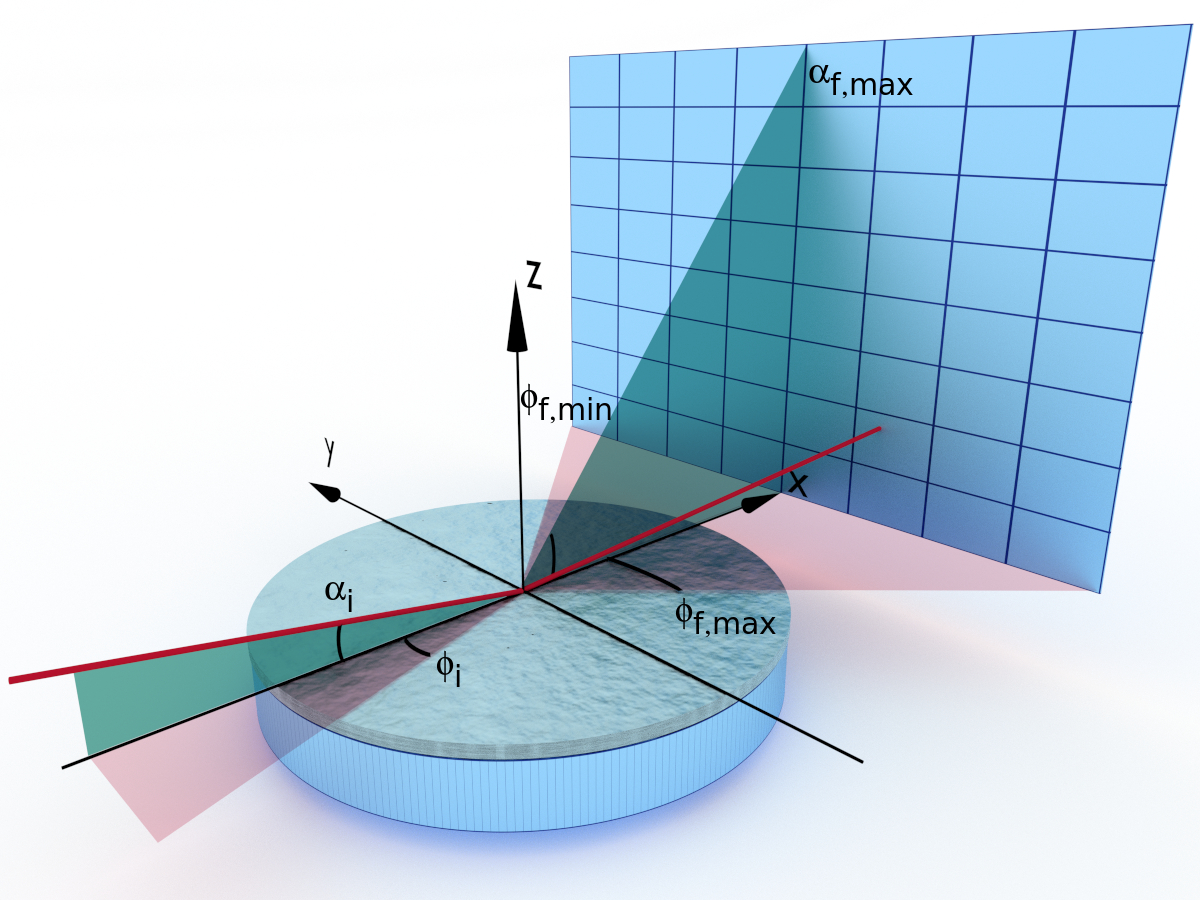
\includegraphics[width=0.6\textwidth]{Figures/BAgeometry_wide}
\end{center}
\caption{The GISAS setup and the coordinate system used in
\BornAgain. The incoming  beam propagates with incidence angles $\alpha_i$ and $\phi_i$ with respect to the sample axes as shown. A scattered (outgoing) beam, characterized by $\alpha_f$ and $\phi_f$ propagates toward the area detector.}
\label{fig:BAsetup_app}
\end{figure}


\begin{itemize}
\item The axis are defined on the interface of the sample with the air. 
The incoming beam points towards the positive $x$-axis direction. The $z$-axis points in the vertical upwards direction (see fig.~\ref{fig:BAsetup_app}).
\item The planes are assumed to be infinite in the planar direction $(x, y)$.
\item The substrate and the air layers are considered infinitely thick.
\item The scattered wave vector is defined as $\mathbf{q}=\mathbf{k}_i-\mathbf{k}_f$
\item The angles $\alpha_i$ and $\alpha_f$ are defined in such a way that those shown in fig.~\ref{fig:BAsetup_app}  are positive.
\item The refractive index of any material is defined as $n=1- \delta + i \beta$, where the values $\delta, \beta \in \mathbb R$ are the inputs used in \BornAgain.
\end{itemize}
Please refer to \SecRef{Simulation} for further details.

\subsection{Default settings}
By default the simulations with \BornAgain\ are performed using the Distorted Wave Born Approximation and the Decoupling Approximation regarding the spatial distribution of particles.


\subsection{Requirements}
\begin{itemize}
  \item The sample is built starting from the top layer.
  \item The particles are always associated with only one layer; they can be deposited on the top surface or buried in the layer. But they cannot cross interfaces.
\end{itemize}
The following sections describe some examples illustrating the main functionalities of \BornAgain .


\newpage
%%%%%%%%%%%%%%%%%%%%%%%%%%%%%%%
\section{Example 1: Cylinders and prisms}
The sample used in this example comprises a substrate on which are deposited, in equal proportion, cylinders and prisms (see fig.~\ref{fig:PythonEx1}(a)). All particles are made of the same material. Each type of particle has the same orientation.

The cylinders are 5~nm high and 5~nm in radius. The prisms are 5~nm high with a triangular base whose side length is equal to 10~nm (see \SecRef{Prism3} and \SecRef{Cylinder} for a description of these form factors). 

There is no interference between the waves scattered by these particles. The distribution is therefore diluted.

The incident neutron beam is characterized by a wavelength of 1~\AA, and incident angles $\alpha_i=0.2^{\circ}$ and $\phi_i=0^{\circ}$.

The simulation is performed using the Distorted Wave Born Approximation. The output intensity generated by this simulation is shown in fig.~\ref{fig:PythonEx1}(b).

\begin{figure}[H]
\hfill
\subfigure[Schematic of the sample]{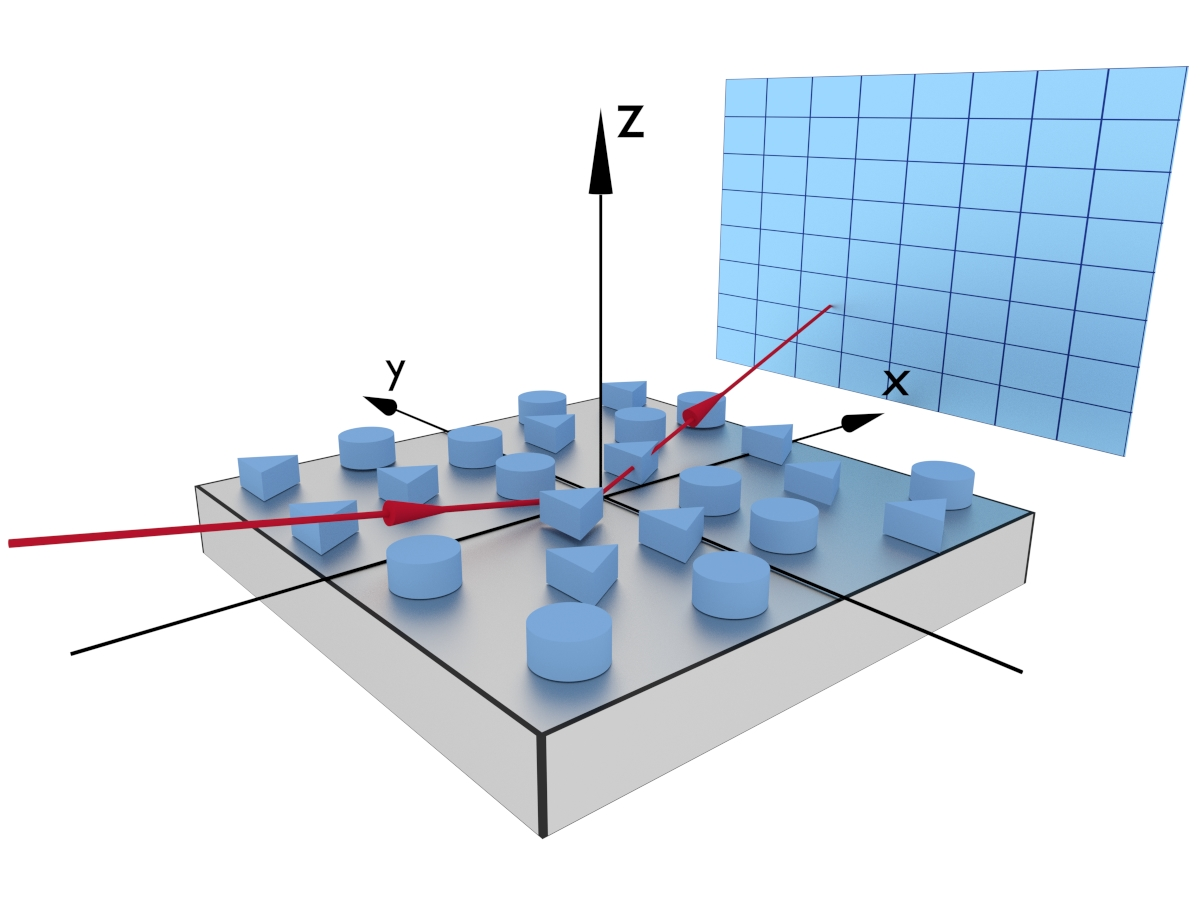
\includegraphics[width=.49\textwidth]{Figures/fig_ex001}}
\hfill
\subfigure[Simulated 2D pattern]{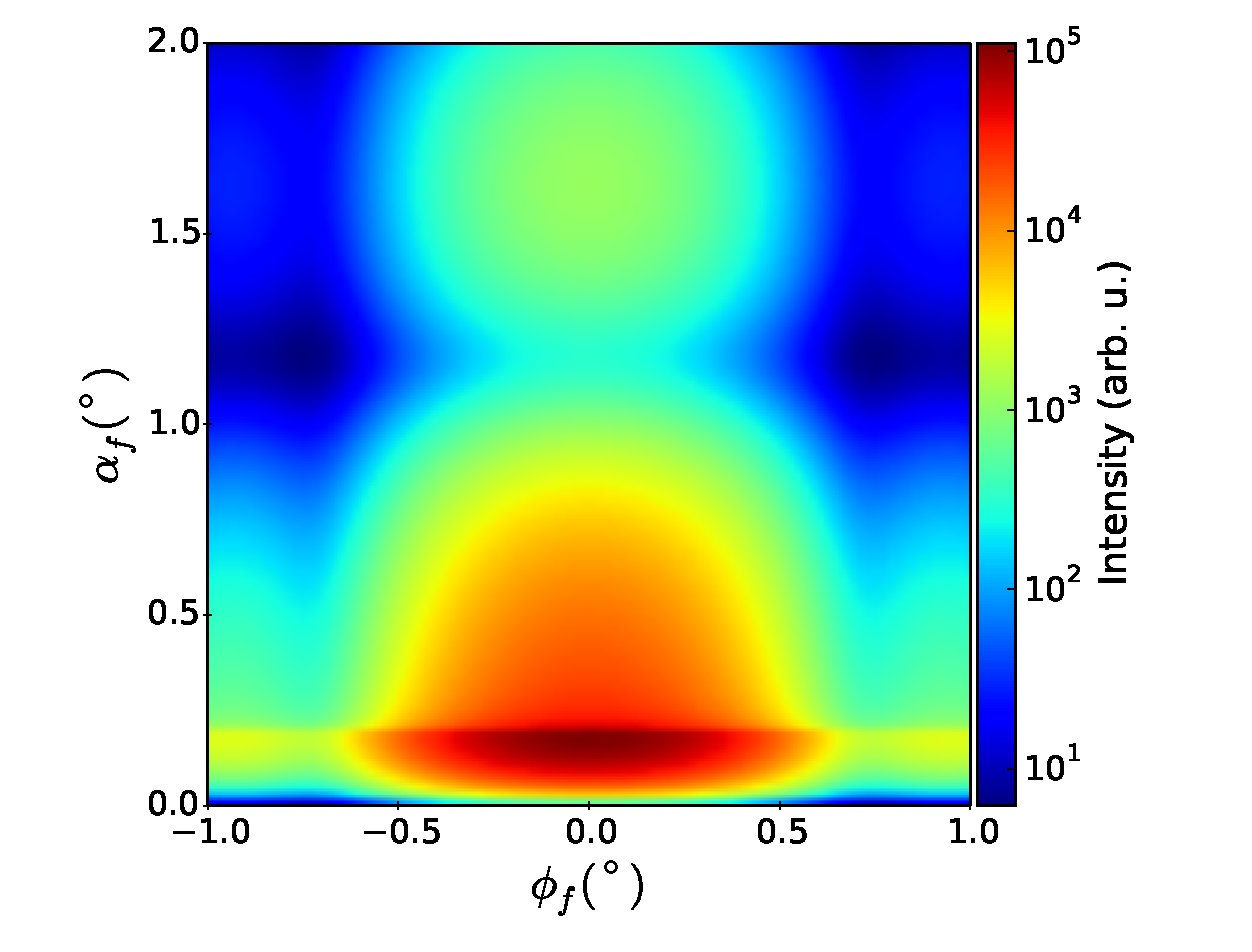
\includegraphics[width=.49\textwidth]{Figures/figure_ex001.eps}}
\hfill
\caption{Example 1: equal proportion of cylinders and prisms3 deposited on a substrate without interference.}
\label{fig:PythonEx1}
\end{figure}

\newpage
%%%%%%%%%%%%%%%%%%%%%%%%%%%%%%%
\section{Example 2: Cylinders with size distribution} \SecLabel{AppPythonEx002}
Here the sample is made of polydisperse cylinders of two different sizes (see fig.~\ref{fig:PythonEx2}(a)). $R_1=H_1$, $R_2=H_2$, where $R_i$ and $H_i$ are the radius and width of cylinder of type $i$.  

There are 95\% of cylinders of type 1 and 5\% of cylinders of type 2.

The polydispersity affects the radii of the cylinders, following a normal distribution. For the small cylinder, their characteristic size varies about $R_1=5$~nm with a standard deviation $\sigma_1=0.2\ R_1$. For type 2, the average value $R_2$ is 10~nm and $\sigma_2=0.02\ R_2$. 

There is no substrate and no interference between the scattered beams.

The simulation is performed using the Born approximation, \textit{i.e.} the sample contains only "air" as a layer without any substrate.

The incident beam is characterized by a wavelength of 1~\AA and incident angles
$\alpha_i=0.2^{\circ}$ and $\phi_i=0^{\circ}$.

The result of the simulation is shown in fig.~\ref{fig:PythonEx2}(b). 

\begin{figure}[H]
\hfill
\subfigure[Schematic of the sample]{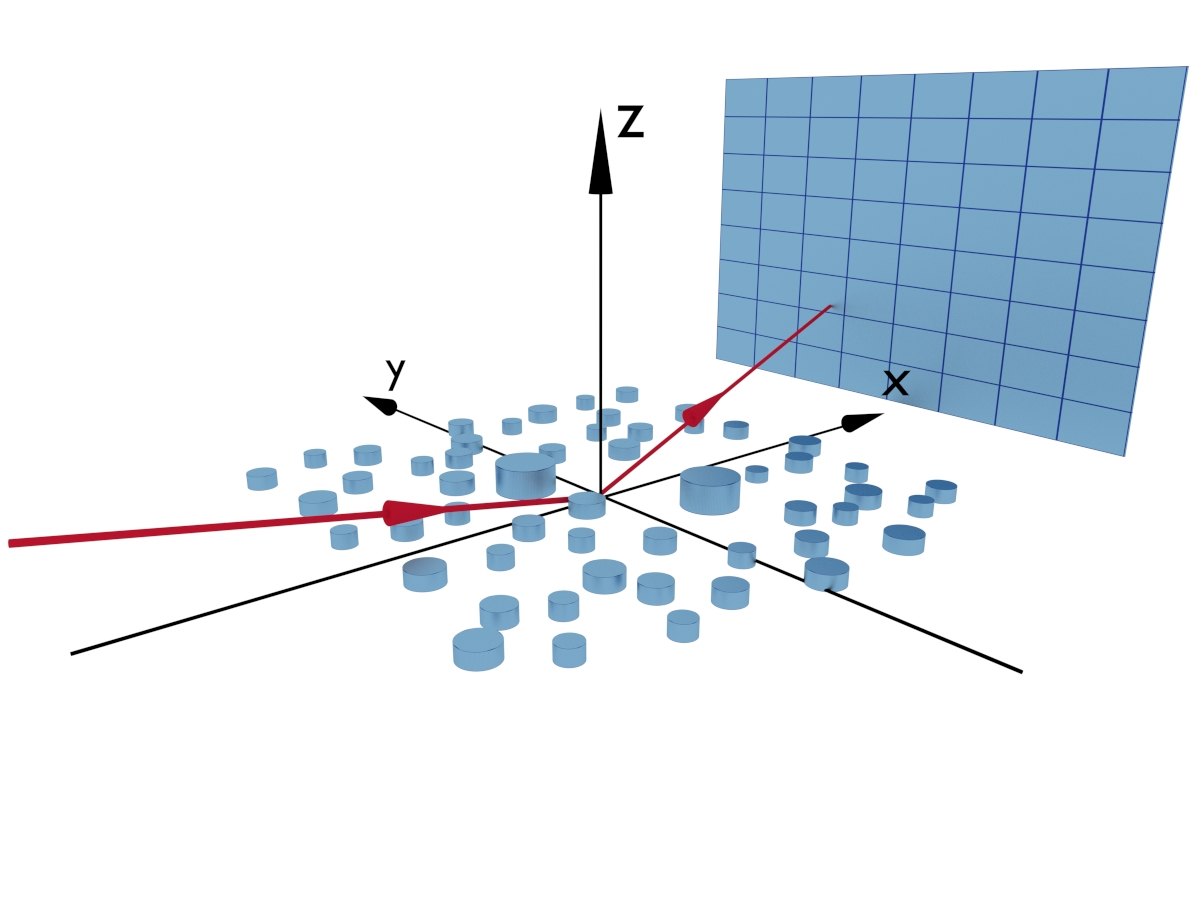
\includegraphics[width=.49\textwidth]{Figures/fig_ex002}}
\hfill
\subfigure[Simulated 2D pattern]{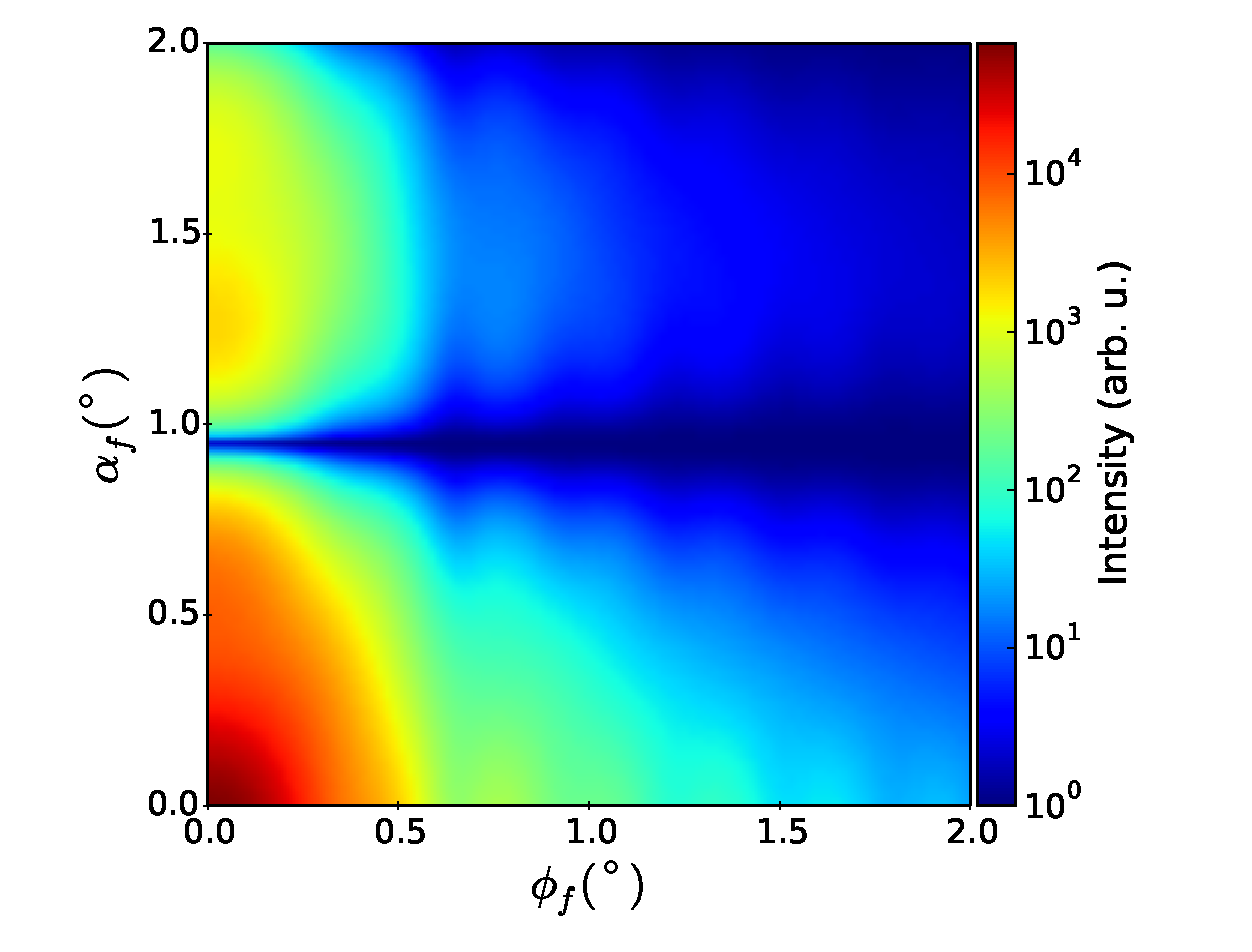
\includegraphics[width=.49\textwidth]{Figures/figure_ex002.eps}}
\hfill
\caption{Example 2: Polydisperse distribution of two types of cylinders.}
\label{fig:PythonEx2}
\end{figure}

\newpage
%%%%%%%%%%%%%%%%%%%%%%%%%%%%%%%
\section{Example 3: "Cylinder" form factor}
This example simulates cylindrical particles in three different configurations.
In each case the wavelength is equal to 1~\AA and the incident angles to $\alpha_i=0.2^{\circ}$, $\phi_i=0^{\circ}$. There is no interference between the scattered waves.

\subsection{Cylindrical form factor in Born approximation} \label{sec:ex003CylinderBA}
The sample considered for this example and the output intensity generated using \BornAgain\ are shown in fig.~\ref{fig:PythonEx3BA}(a) and (b), respectively. The cylinders are all identical with a radius and height equal to 5~nm. The simulation is performed in the Born approximation, by using only the air layer (no substrate).

\begin{figure}[H]
\hfill
\subfigure[Schematic of the sample]{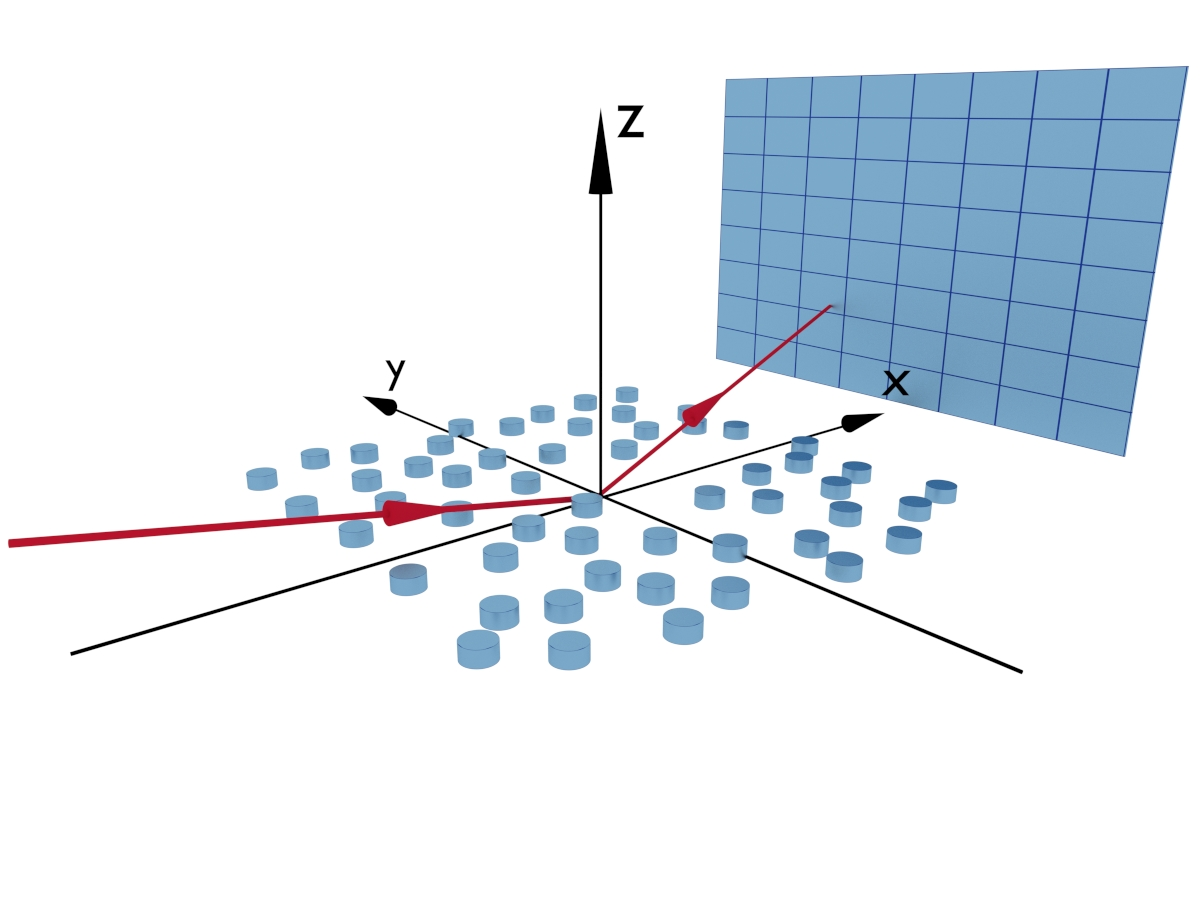
\includegraphics[width=.49\textwidth]{Figures/fig_ex003BA}}
\hfill
\subfigure[Simulated 2D pattern]{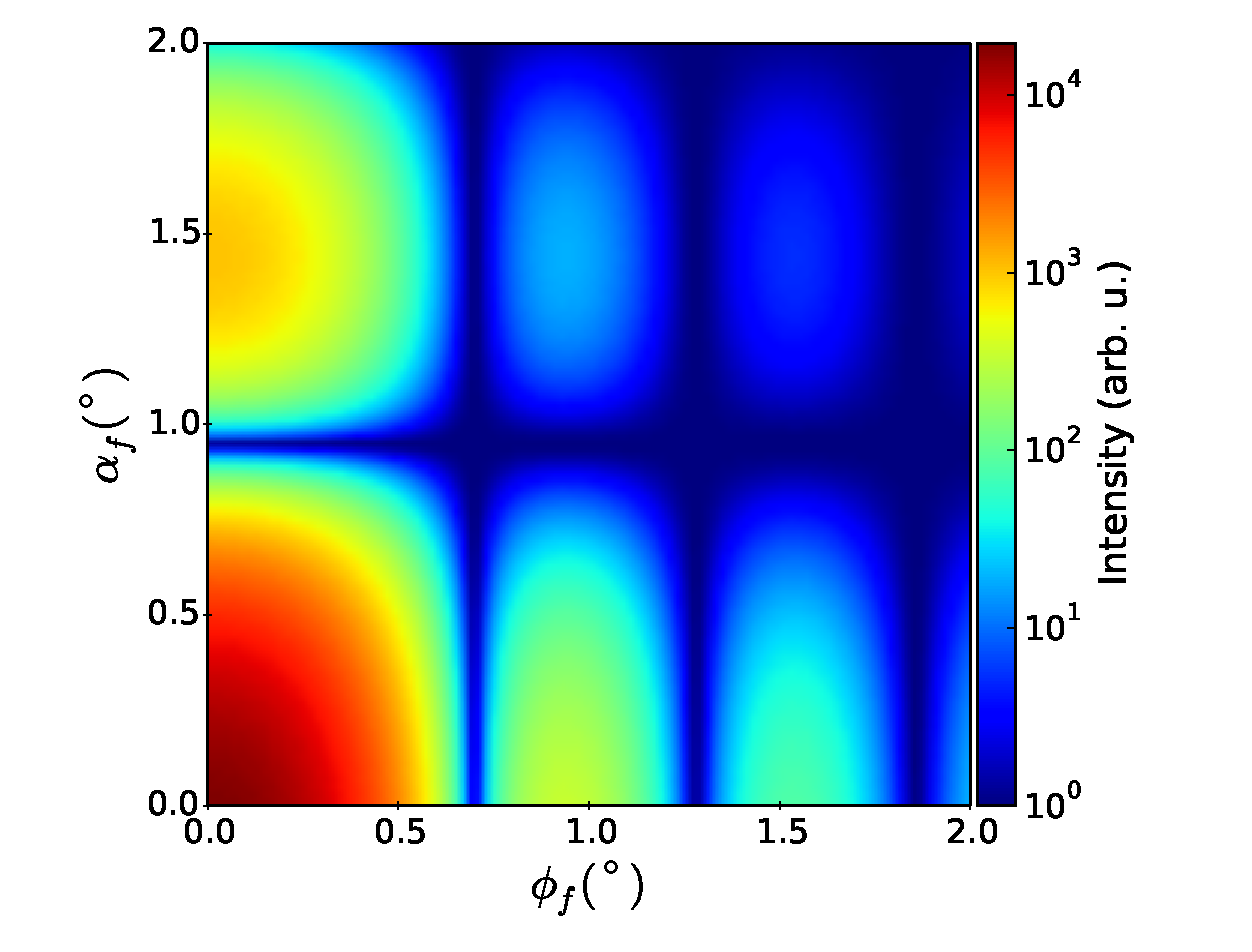
\includegraphics[width=.49\textwidth]{Figures/figure_ex003BA.eps}}
\hfill
\caption{Example 3: Scattering from a monodisperse distribution of cylinders using the Born approximation.}
\label{fig:PythonEx3BA}
\end{figure}

\subsection{Cylindrical form factor in the Born approximation with size distribution}
This example considers a polydisperse distribution of cylinders (see fig.~\ref{fig:PythonEx3BASize}(a)). Their average radii and heights are equal to 5~nm. The radii of the cylinders vary according to a normal distribution with a standard deviation $\sigma$ equal to 0.2 times the average radius. The simulated output pattern is shown in fig.~\ref{fig:PythonEx3BASize}(b).

\begin{figure}[H]
\hfill
\subfigure[Schematic of the sample]{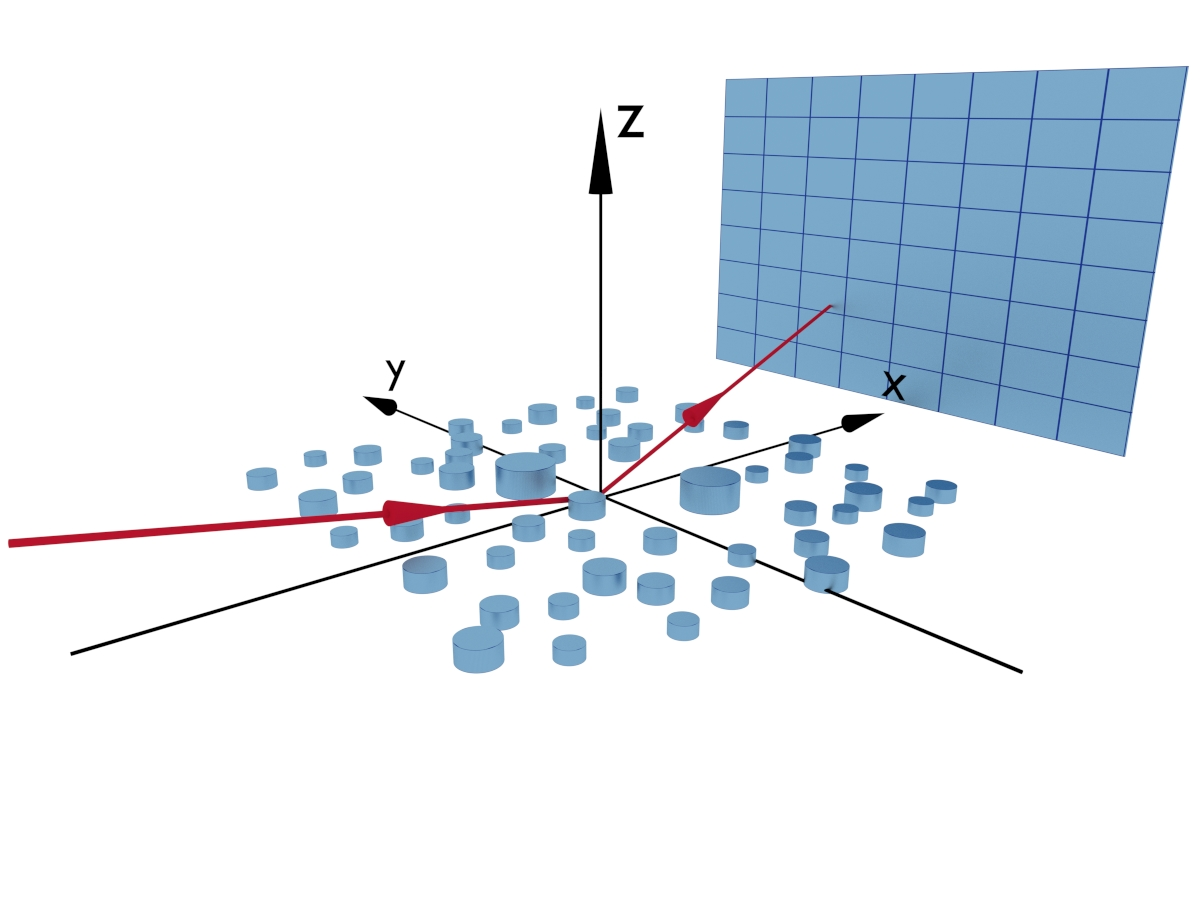
\includegraphics[width=.49\textwidth]{Figures/fig_ex003BASize}}
\hfill
\subfigure[Simulated 2D pattern]{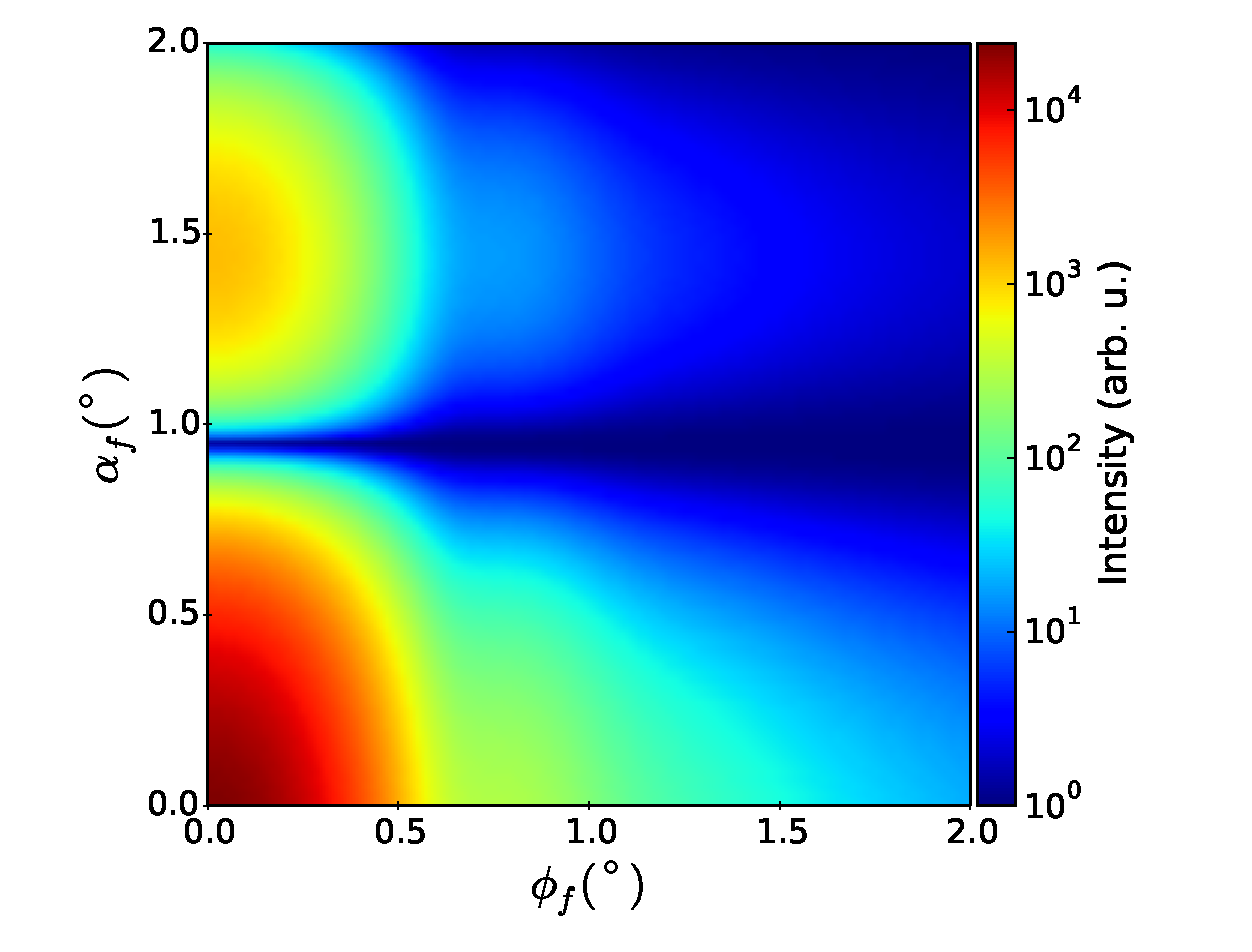
\includegraphics[width=.49\textwidth]{Figures/figure_ex003BASize.eps}}
\hfill
\caption{Example 3: Scattering from a polydisperse distribution of cylinders using the Born approximation.}
\label{fig:PythonEx3BASize}
\end{figure}


\MakeRemark{Remark:}{ \\
This example differs from the one described in \SecRef{AppPythonEx002} by the presence of a single distribution of cylinders.}


\subsection{Cylindrical form factor in DWBA} \label{sec:ex003CylinderDWBA}
This example is similar to the case with  the Born Approximation (Section \ref{sec:ex003CylinderBA}) with the addition of a substrate (see fig.~\ref{fig:PythonEx3DWBA})(a)). Therefore the Distorted Wave Born Approximation is implemented in order to take additional reflections and transmission at the substrate interface into account.
The distribution of cylinders is monodisperse with a height and a radius of 5~nm.

\begin{figure}[H]
\hfill
\subfigure[Schematic of the sample]{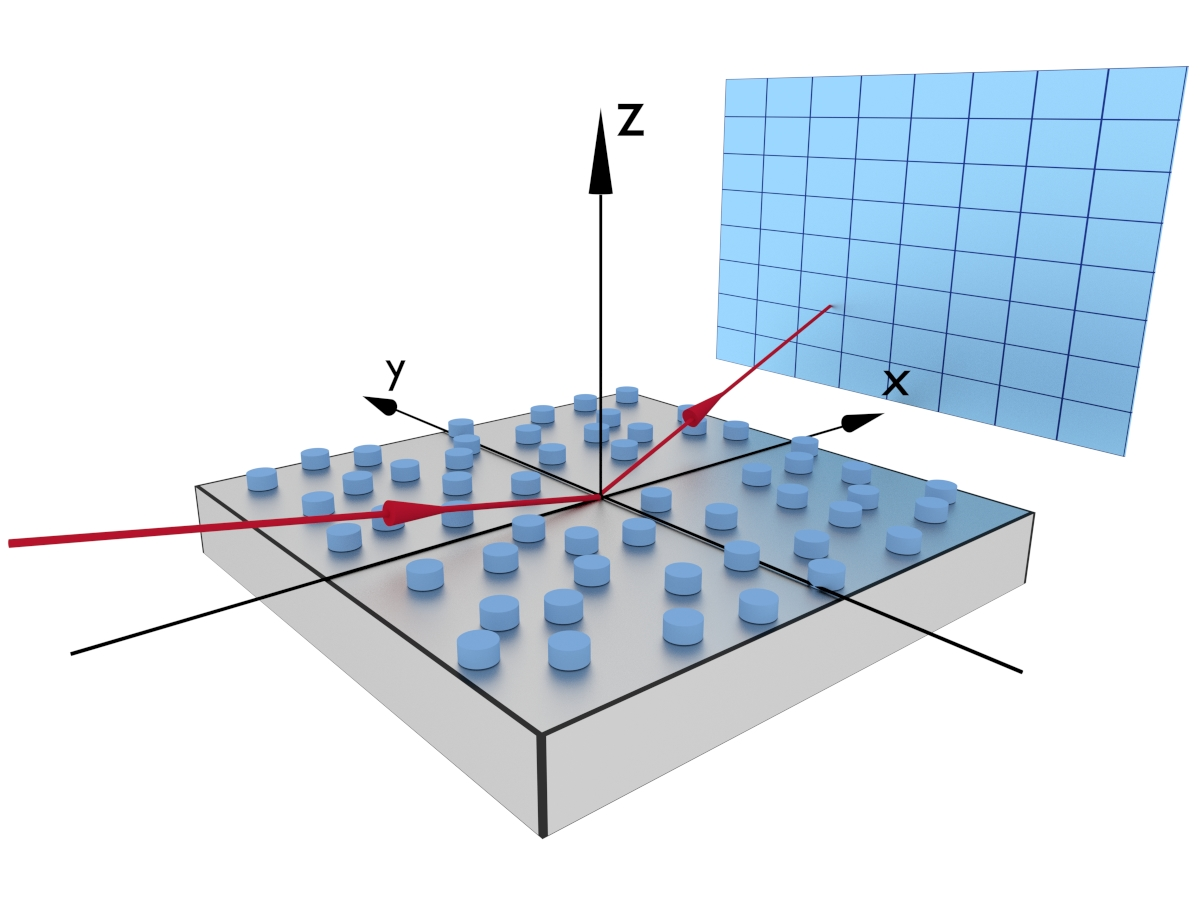
\includegraphics[width=.49\textwidth]{Figures/fig_ex003DWBA}}
\hfill
\subfigure[Simulated 2D pattern]{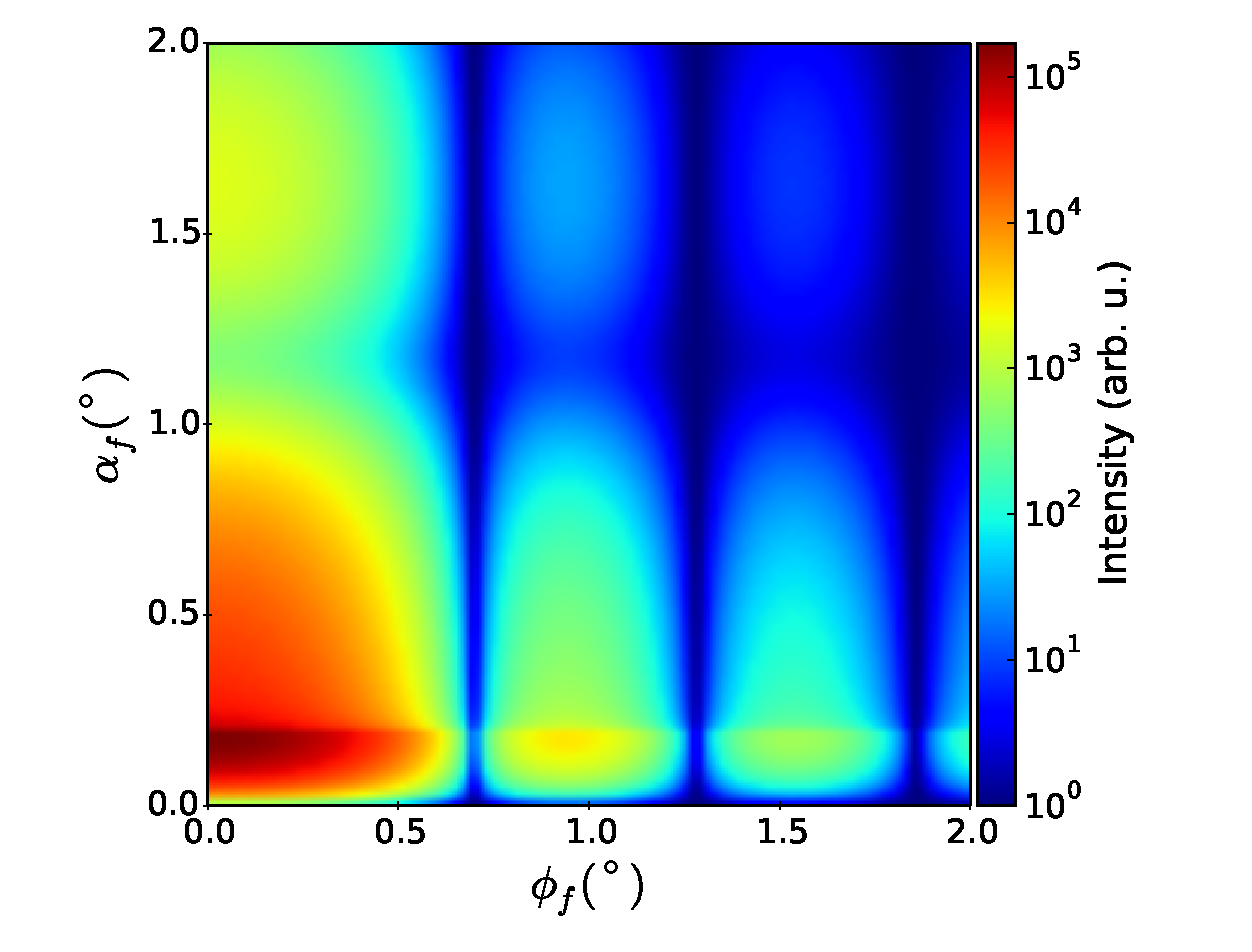
\includegraphics[width=.49\textwidth]{Figures/figure_ex003DWBA.eps}}
\hfill
\caption{Example 3: Scattering from a monodisperse distribution of cylinders deposited on a substrate using the Distorted Wave Born approximation.}
\label{fig:PythonEx3DWBA}
\end{figure}

\newpage
%%%%%%%%%%%%%%%%%%%%%%%%%%%%%%%
\section{Example 4: Cylinders - Paracrystal}
The example focuses on the planar distribution of particles. Two cases are considered: a one- and a two-dimensional paracrystal. 
The two examples of this section share the following settings:
\begin{itemize}
\item The incident beam is characterized by a wavelength of 1~\AA and angles $\alpha_i=0.2^{\circ}$ and $\phi_i=0^{\circ}$.
\item The particles are cylinders with constant radii and heights equal to 5~nm. They are deposited on a substrate.
\end{itemize}

\subsection{"One dimension"}
The disorder is radially propagated. It is characterized by a Gaussian distribution $\exp(-\omega^2q^2/2)$ with $\omega=7$~nm.\\ The average distance between the particles $D$ is equal to  20~nm.\\ Finite size effects are modelled by introducing a damping length $\Gamma$ equal to 1e3~nm.\\
In this case, the structure factor is given by

\begin{equation*}
S(q_{\parallel})= \frac{1-\phi^2 }{1-2\phi\cos(q_{\parallel} D)+\phi^2} \; \textrm{with} \ \phi=\exp(-\omega^2 q_{\parallel}^2/2)\exp(-D/\Gamma).
\end{equation*}
%Its Fourier transform, the pair correlation function $g(r)$, is plotted in fig.~\ref{fig:PythonEx41DDL}a).


\begin{figure}[H]
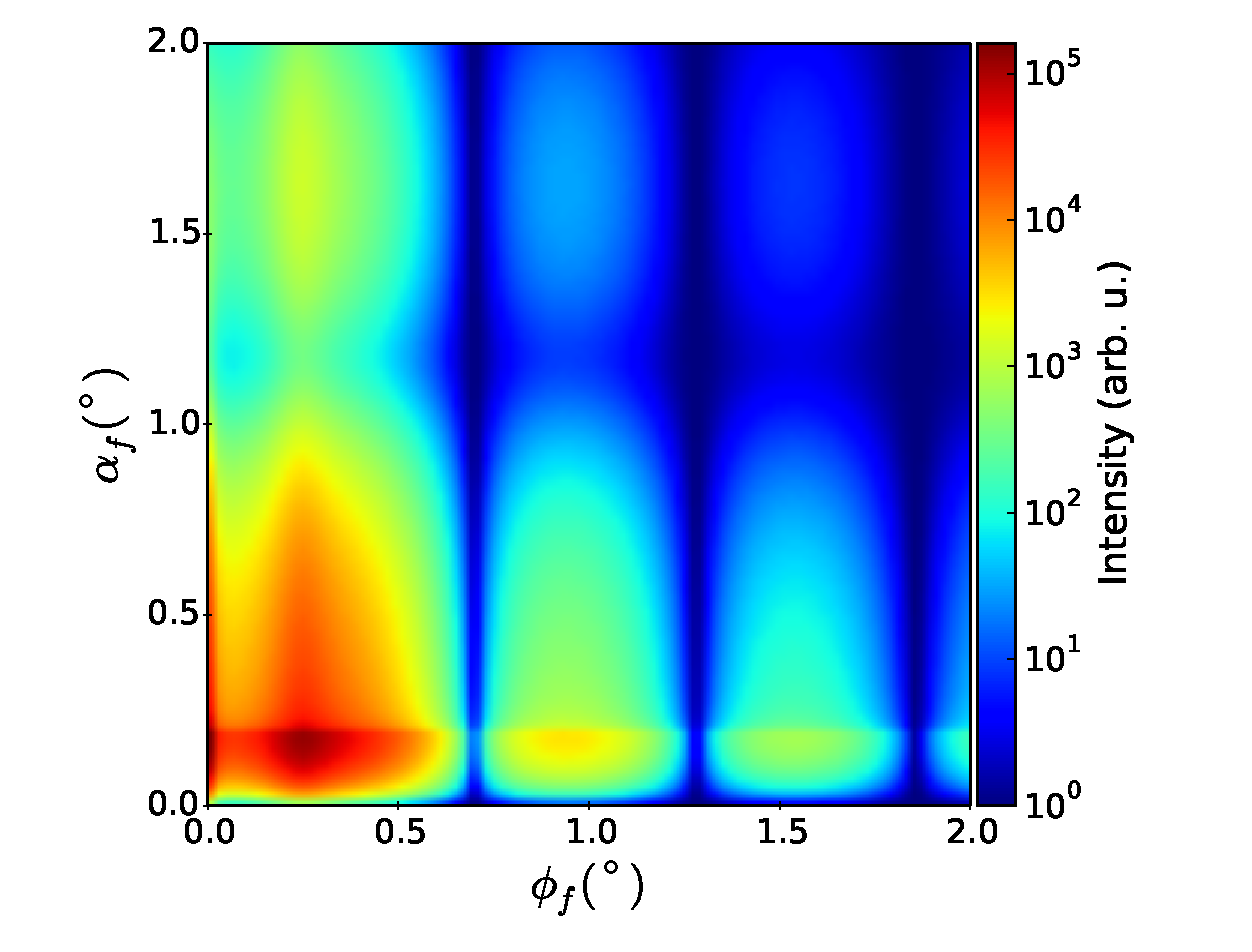
\includegraphics[width=.49\textwidth]{Figures/figure_ex0041DDL.eps}
\caption{Example 4 - One dimension : Scattering from a distribution of cylinders deposited on a substrate using the Distorted Wave Born approximation, distribution according to a radial paracrystal.}
\label{fig:PythonEx41DDL}
\end{figure}

%\begin{figure}[H]
%\hfill
%\subfigure[Pair distribution function as function of radial coordinate]{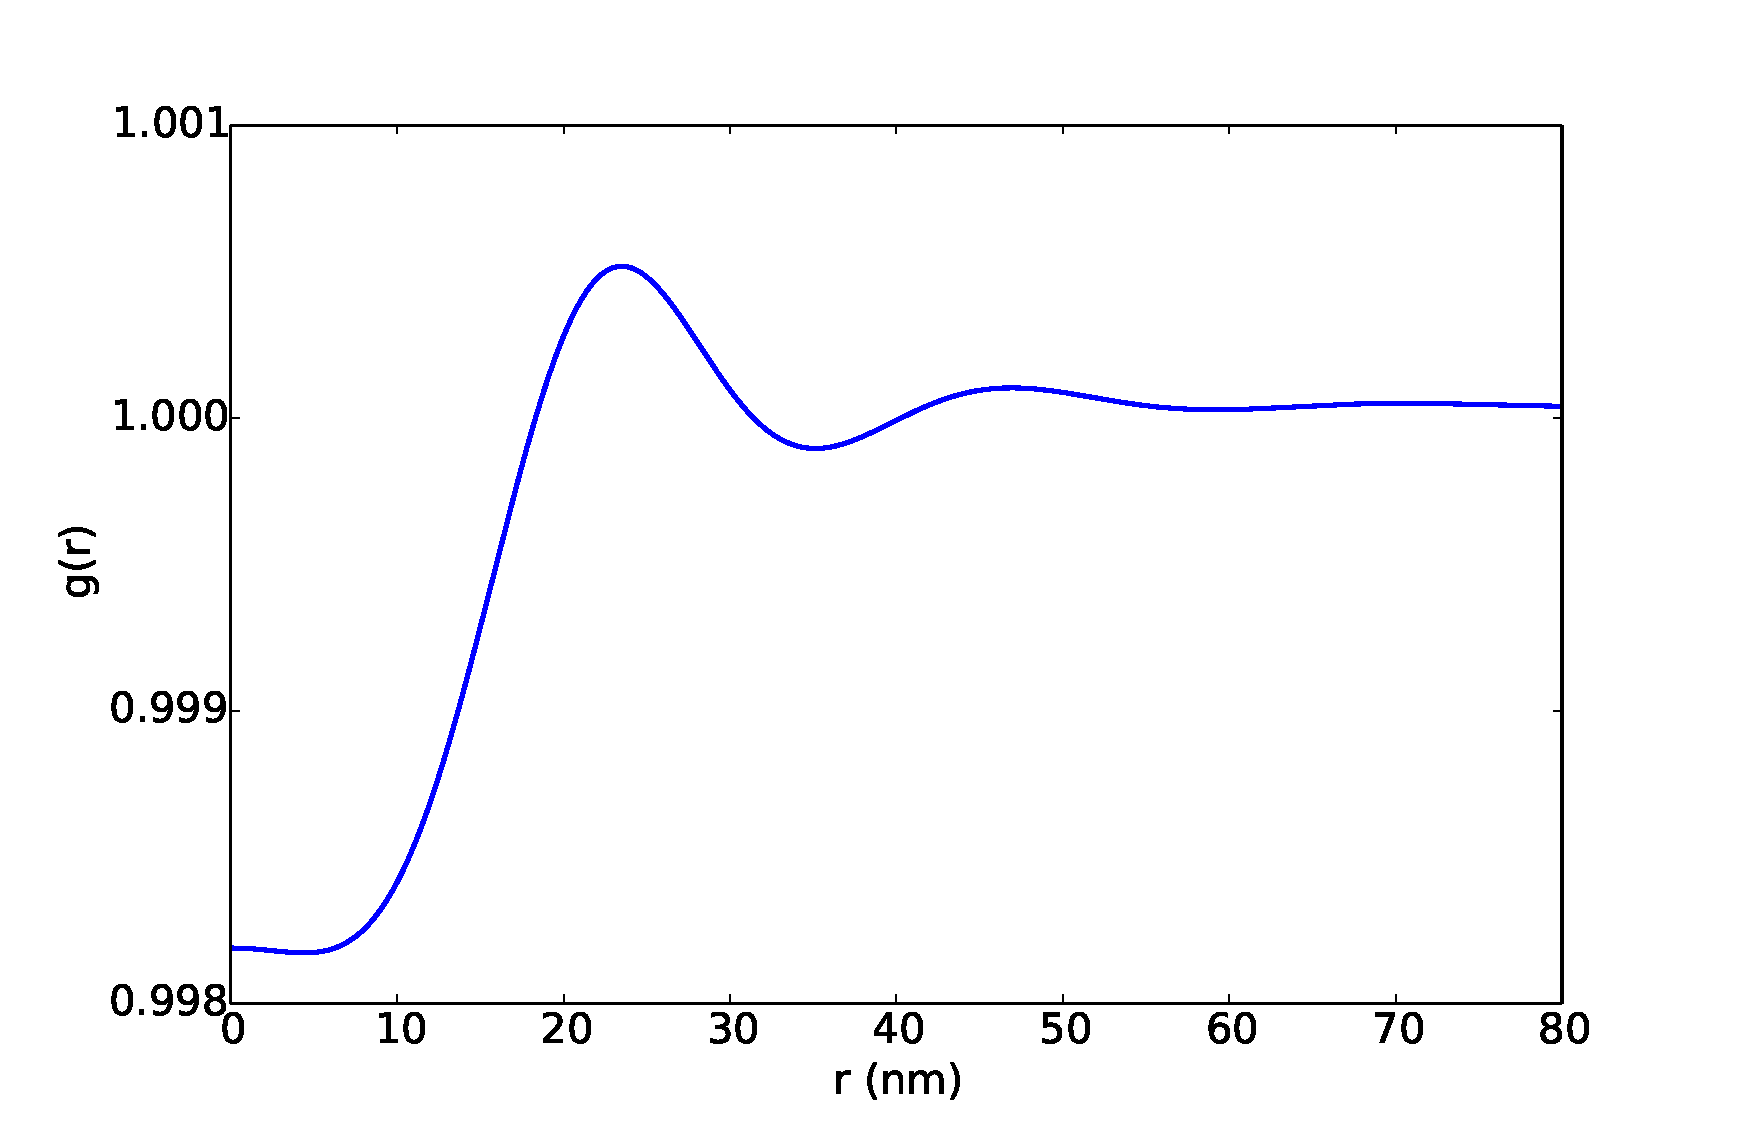
\includegraphics[width=.49\textwidth]{Figures/g_r_1dpara.eps}}
%\hfill
%\subfigure[Simulated 2D pattern]{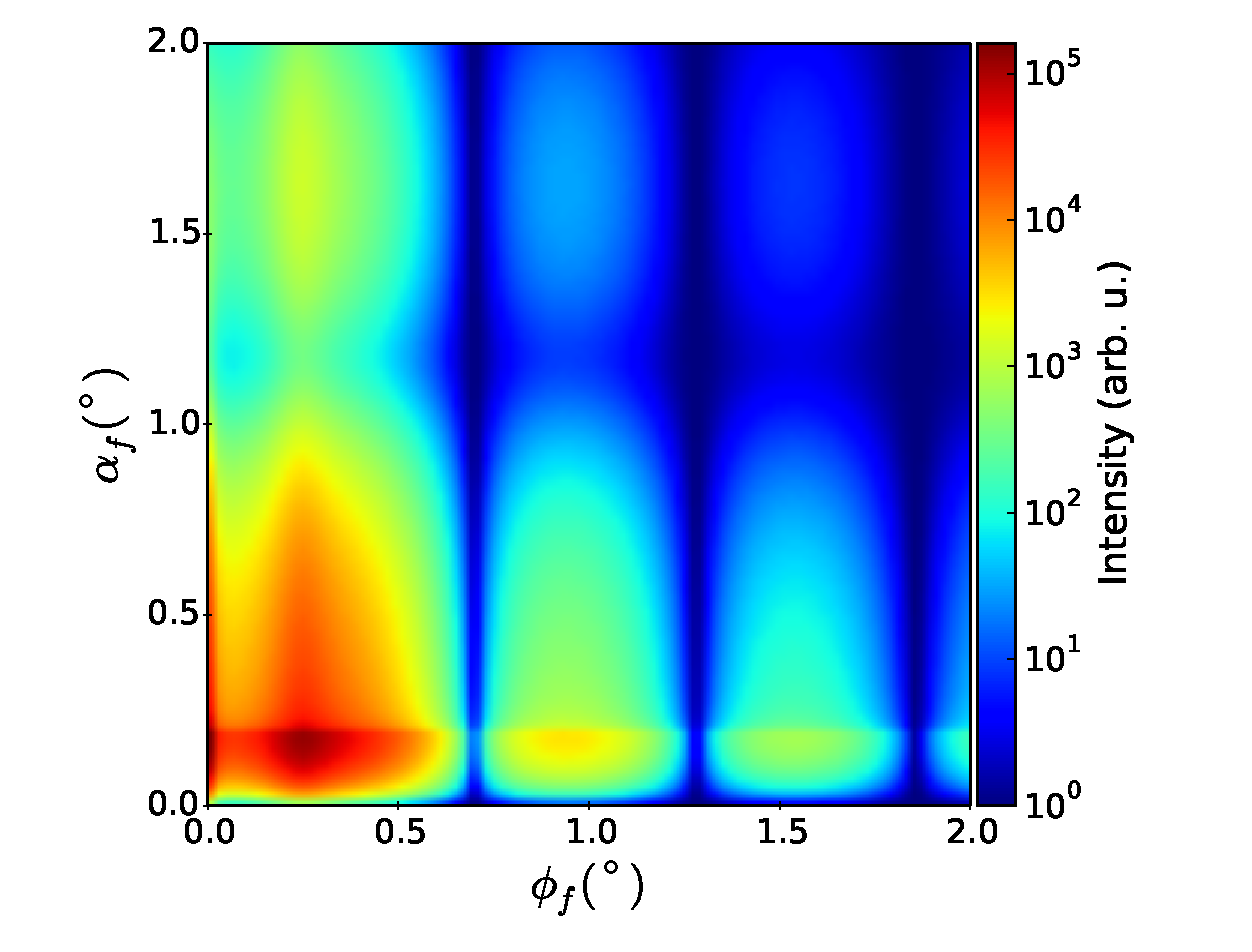
\includegraphics[width=.49\textwidth]{Figures/figure_ex0041DDL.eps}}
%\hfill
%\caption{Example 4 - One dimension : Scattering from a distribution of cylinders deposited on a substrate using the Distorted Wave Born approximation, distribution according to a radial paracrystal.}
%\label{fig:PythonEx41DDL}
%\end{figure}

\subsection{Two dimensions}
The cylindrical particles are distributed along a square lattice whose order is gradually distorted.
The average distance between the particles is 20~nm. The size of the domains is 20~$\mu$m in both directions.

The distribution function is a two-dimensional Cauchy function with correlation lengths equal to 1~nm in both directions.


\begin{figure}[H]
\hfill
\subfigure[Schematic of the sample]{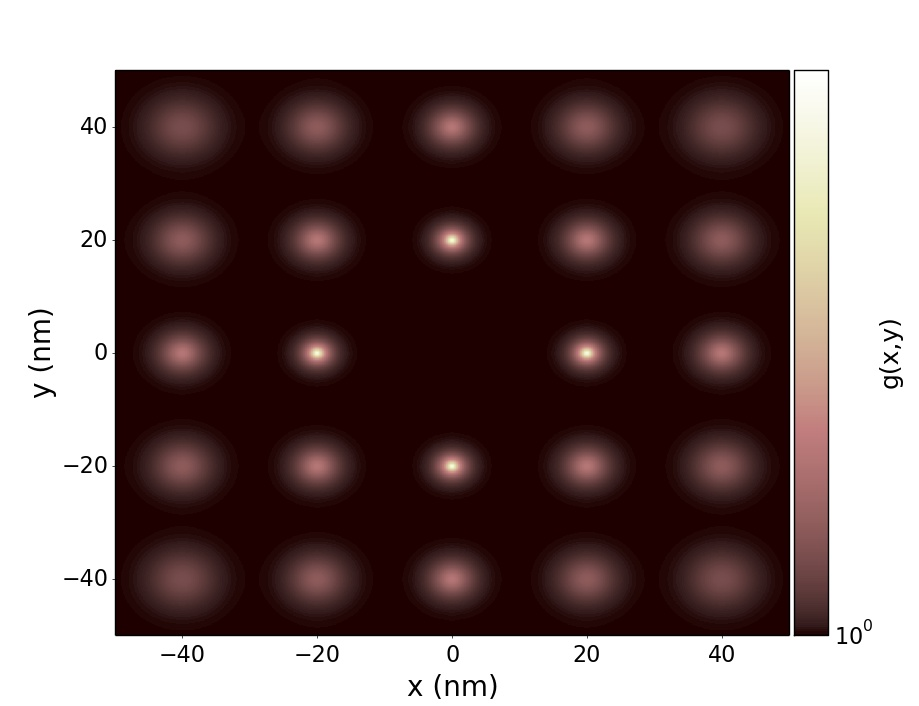
\includegraphics[width=.49\textwidth]{Figures/g_r_2dparasq}}
\hfill
\subfigure[Simulated 2D pattern]{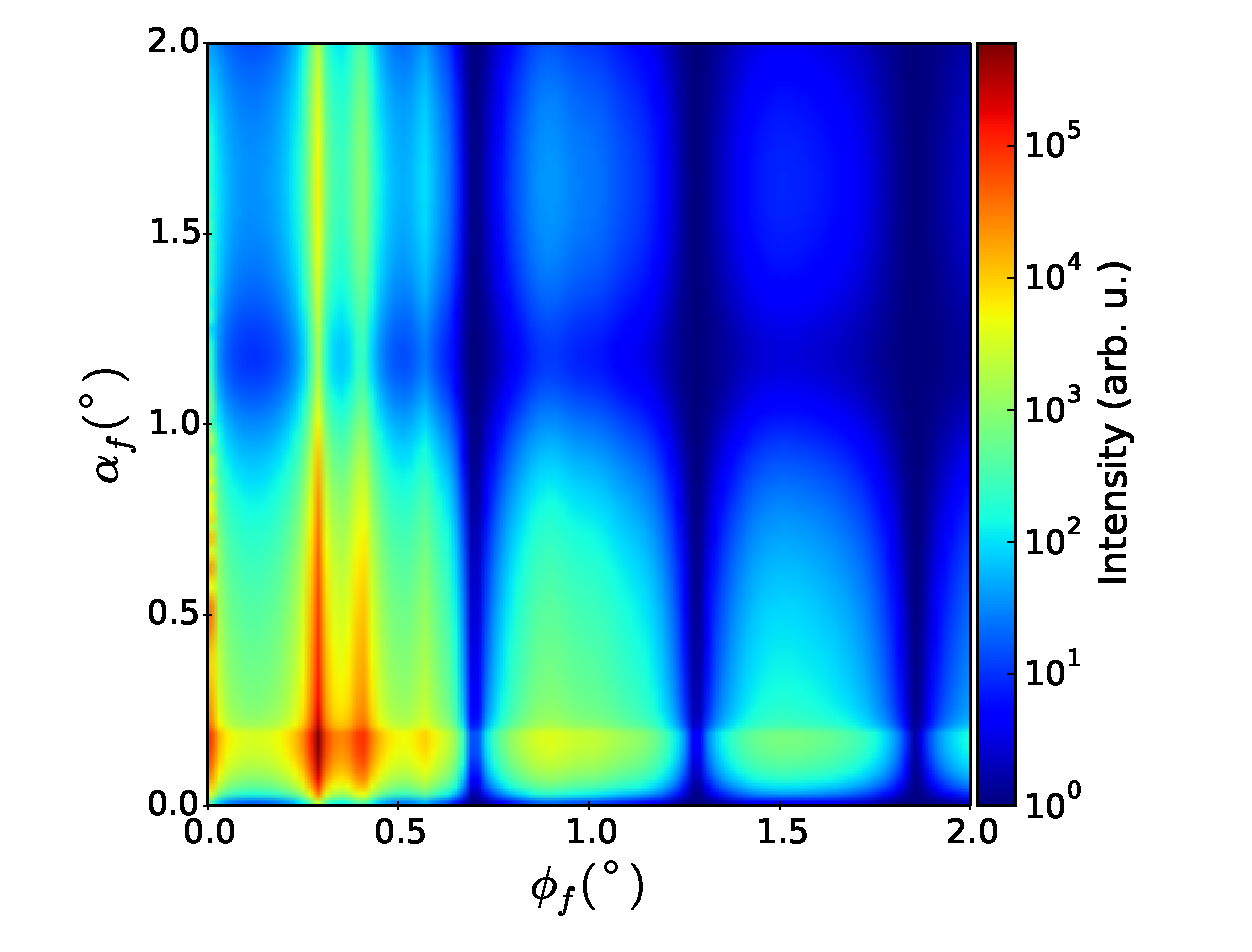
\includegraphics[width=.49\textwidth]{Figures/figure_ex0042DDLsq.eps}}
\hfill
\caption{Output ex004 2DDL.}
%\label{}
\end{figure}

\newpage
%%%%%%%%%%%%%%%%%%%%%%%%%%%%%%%
\section{Example 5: Lattice with disorder}
The examples of this section focus on the available options to characterize the pattern according to which the particles are deposited.


\subsection{Disorder 1} \label{sec:ex005Dis1}
Cylinders with radii and heights of 3~nm are deposited on a substrate (fig.~\ref{fig:PythonEx5Dis1}(a)). They are distributed along a square lattice with a lattice length of 25~nm, whose one of the main axes is parallel to the $x$-axis. The lattice is initialized by placing a cylinder at the origin.\\ The rod shape distribution is a two-dimensional Cauchy function in reciprocal space with anisotropic correlation lengths equal to $cl_x=300/(2\pi)$~nm and $cl_y=100/(2\pi)$~nm.
%The probability distribution function is a two-dimensional Cauchy function  with anisotropic correlation lengths equal to $cl_x=300/(2\pi)$~nm and $cl_y=100/(2\pi)$~nm.


The incident beam is characterized by a wavelength of 1~\AA and angles $\alpha_i=0.2^{\circ}$ and $\phi_i=0^{\circ}$.
 
The simulation is run using the DWBA.

% question: LMA with constant size of particles?? 
\begin{figure}[H]
\hfill
\subfigure[Schematic of the sample]{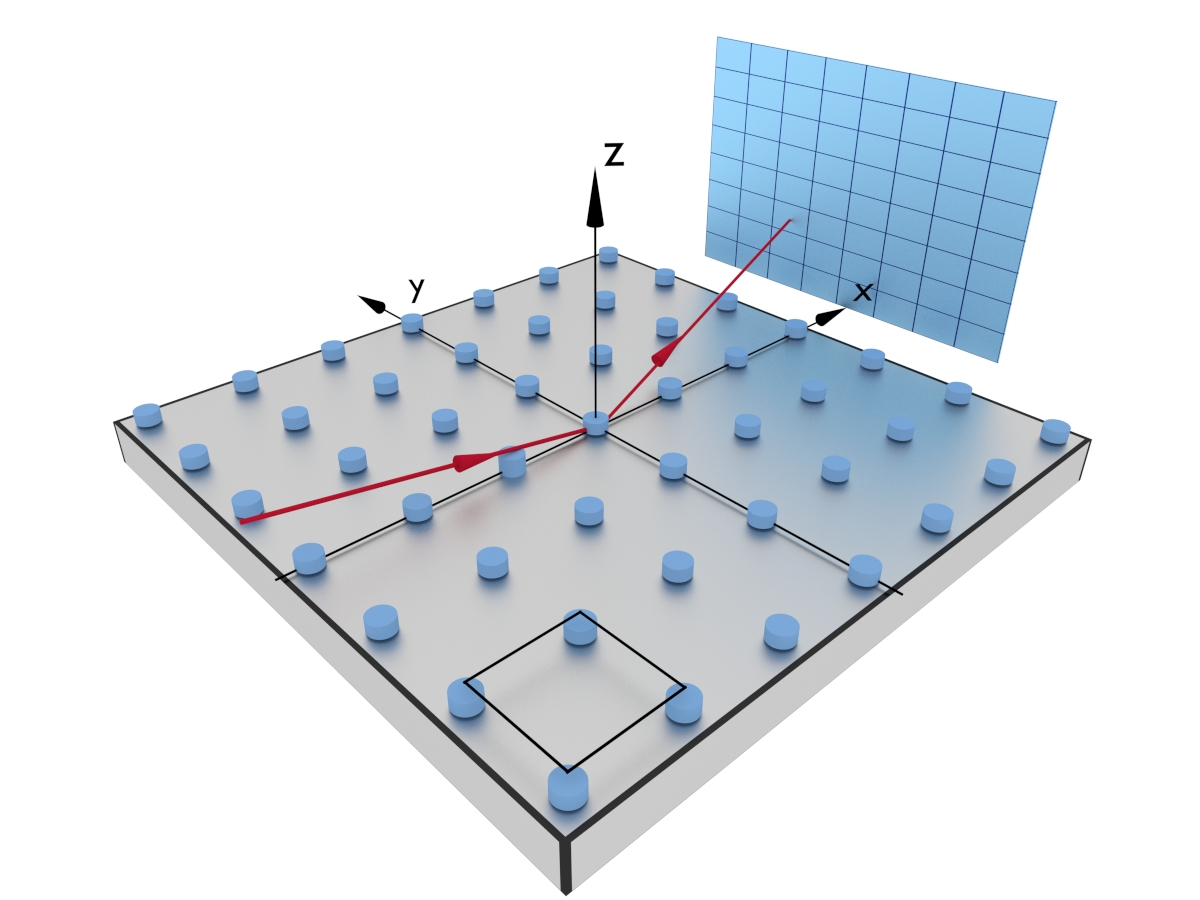
\includegraphics[width=.49\textwidth]{Figures/fig_ex005Dis1}}
\hfill
\subfigure[Simulated 2D pattern]{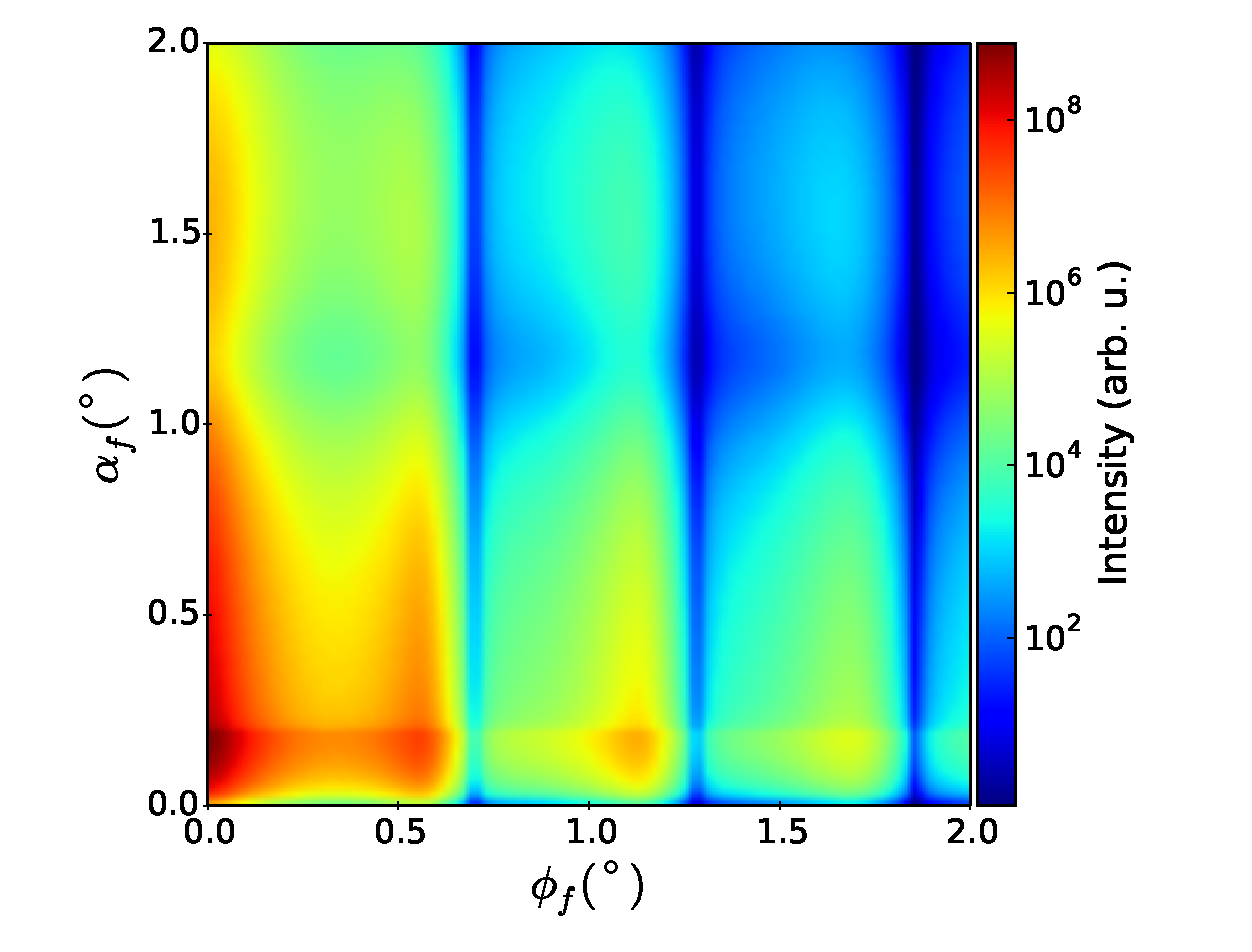
\includegraphics[width=.49\textwidth]{Figures/figure_ex005Disorder1.eps}}
\hfill
\caption{Example 005 - Disorder1: Scattering from a monodisperse distribution of cylinders deposited on a substrate along a squared lattice using the Distorted Wave Born approximation.}
\label{fig:PythonEx5Dis1} 
\end{figure}

\subsection{Disorder 2}
This sample differs from the previous one by an overlap of two spatial distributions of cylinders. The first square lattice is centered at the origin. The second one, with the same lattice spacing and the same cylinders at the nodes is initialized at $x=y=12.5$~nm.

\begin{figure}[H]
\hfill
\subfigure[Schematic of the sample]{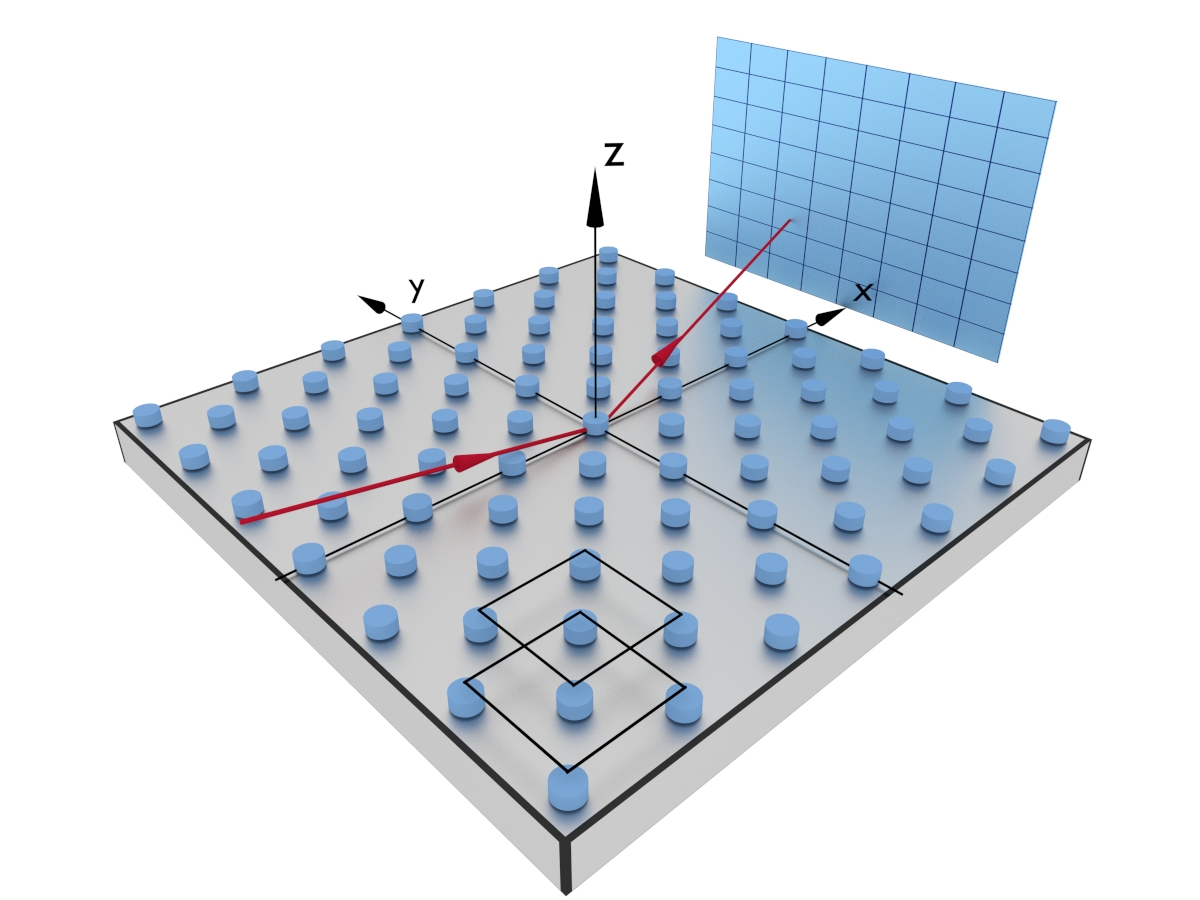
\includegraphics[width=.49\textwidth]{Figures/fig_ex005Dis2}}
\hfill
\subfigure[Simulated 2D pattern]{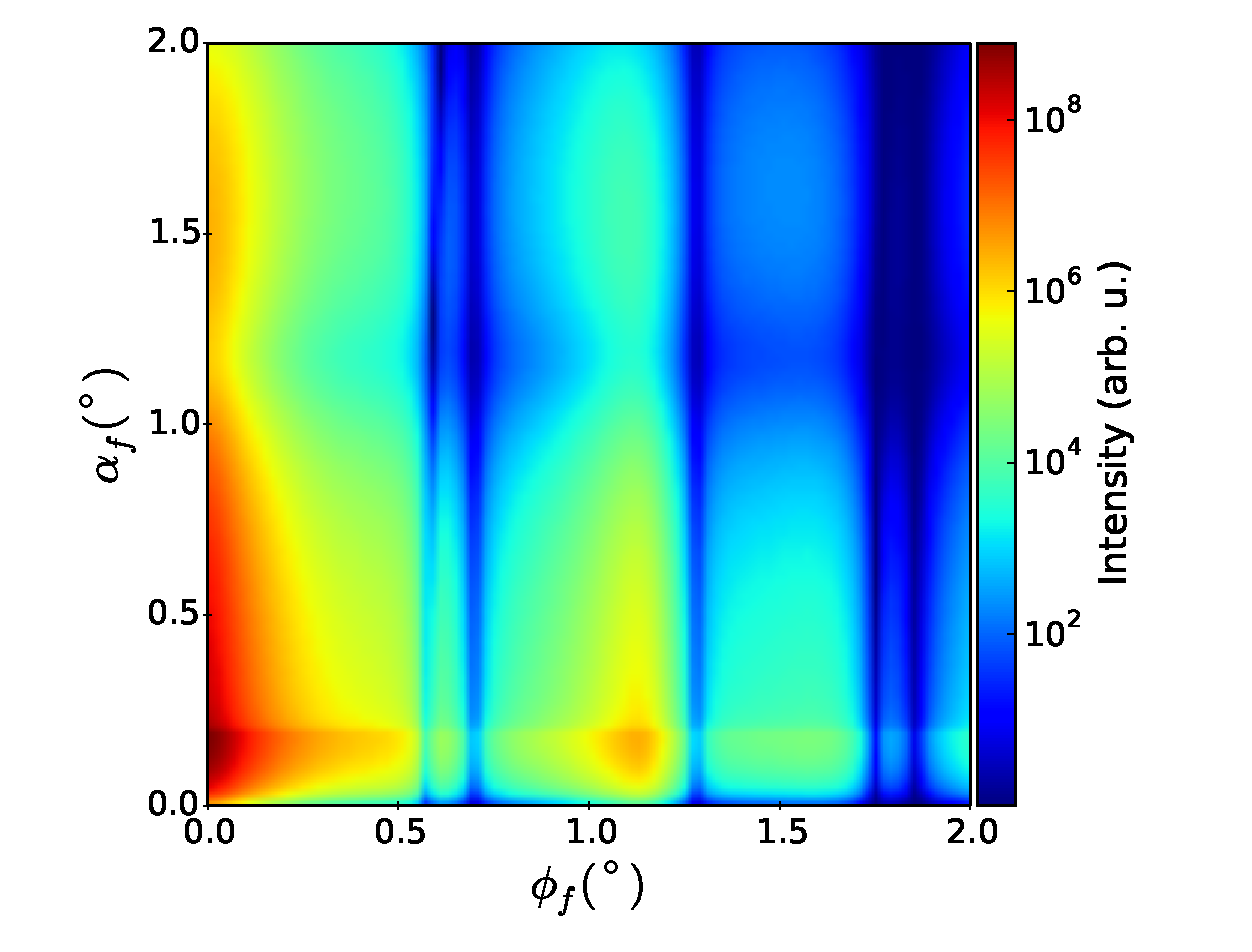
\includegraphics[width=.49\textwidth]{Figures/figure_ex005Disorder2.eps}}
\hfill
\caption{Example 005 - Disorder2: Scattering from two monodisperse distributions of cylinders deposited on a substrate along a squared lattice using the Distorted Wave Born approximation. One of the lattices is laterally offset with respect to the other by 12.5~nm along the $x-$ and $y-$ axes.}
\label{fig:PythonEx5Dis2} 
\end{figure}

\subsection{Disorder 3}
Compared to Section~\ref{sec:ex005Dis1}, the square lattice used in this example is now rotated with respect to the main referential by $30^{\circ}$. Note that the axes of the rod shape's distribution are also rotated using \Code{setGamma}.



\begin{figure}[H]
\hfill
\subfigure[Schematic of the sample]{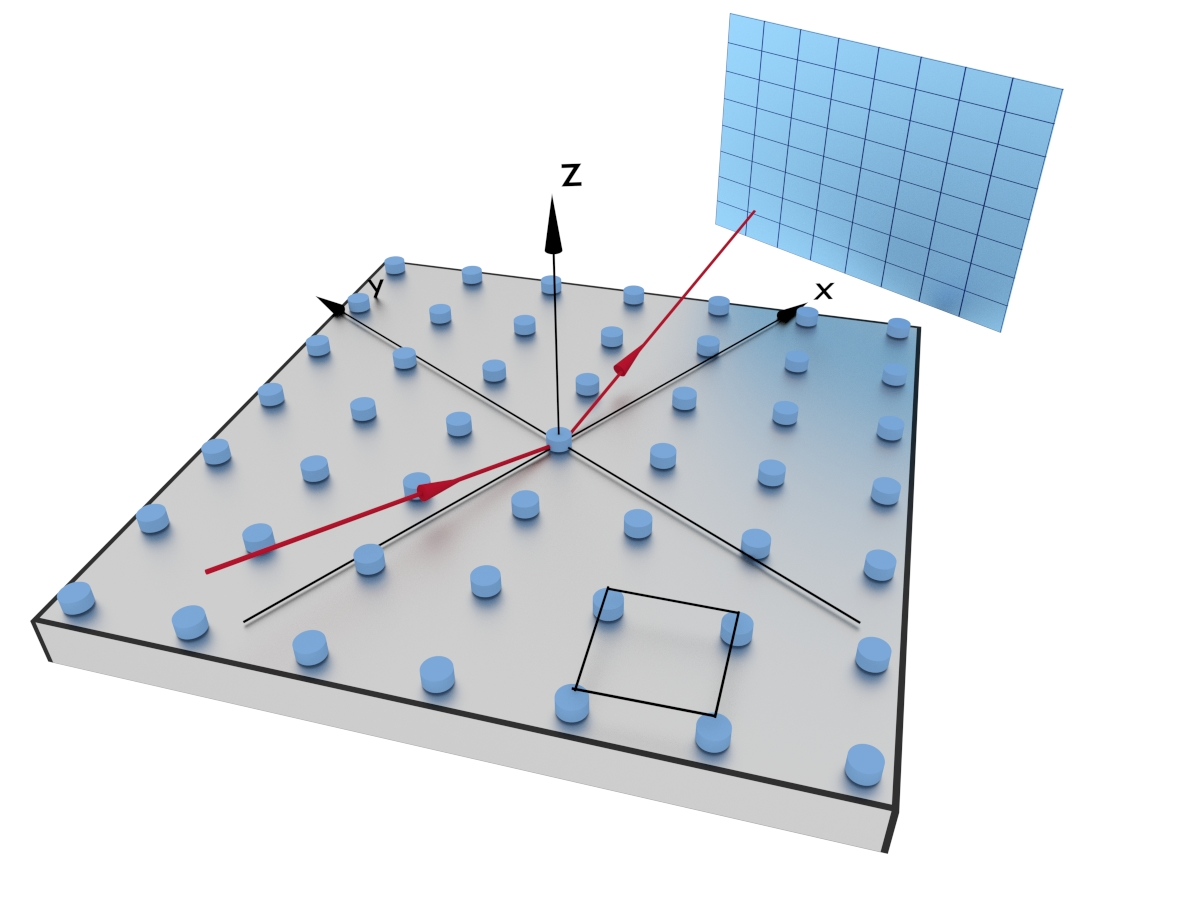
\includegraphics[width=.49\textwidth]{Figures/fig_ex005Dis3}}
\hfill
\subfigure[Simulated 2D pattern]{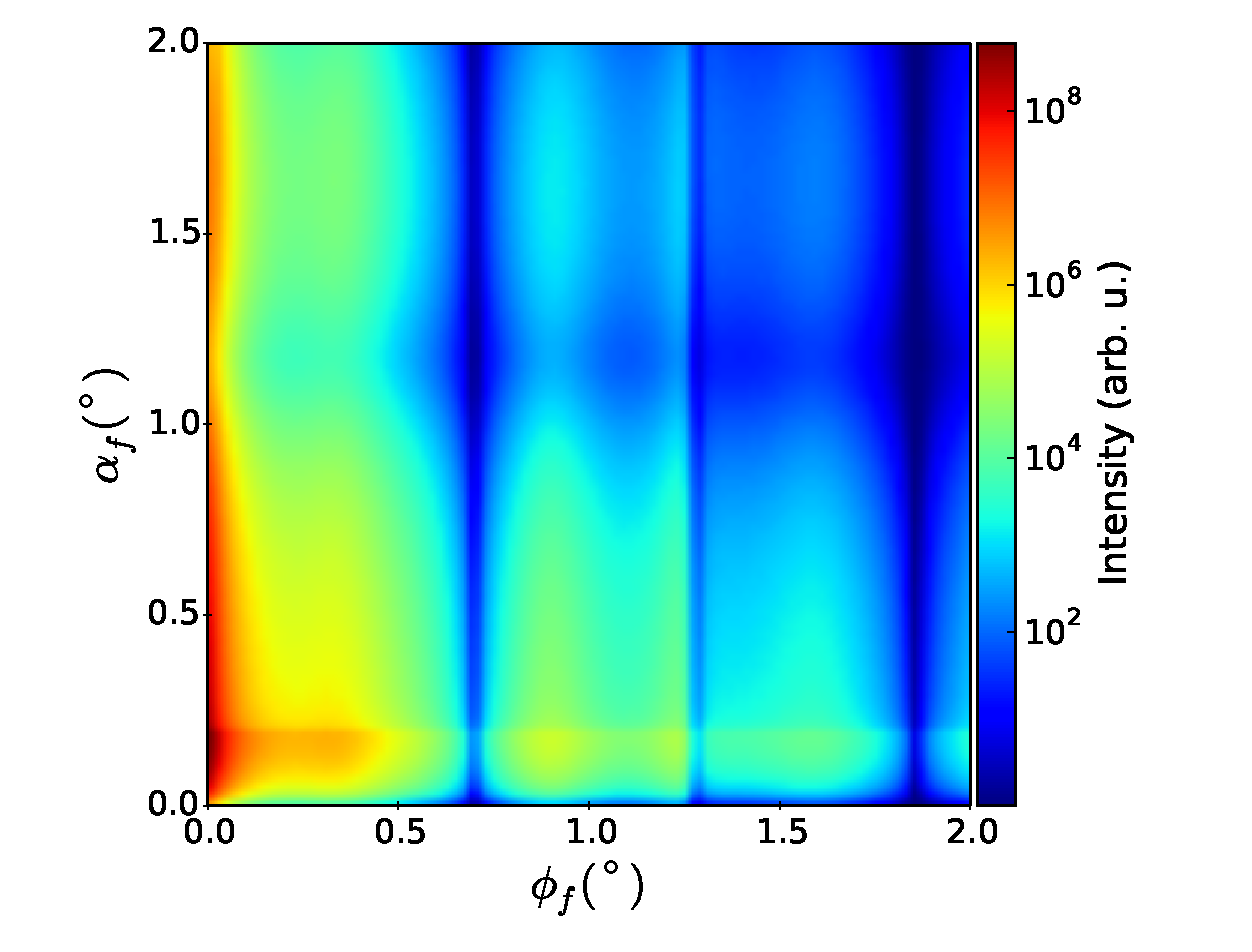
\includegraphics[width=.49\textwidth]{Figures/figure_ex005Disorder3.eps}}
\hfill
\caption{Example 005 - Disorder3: Scattering from a monodisperse distribution of cylinders deposited on a substrate along a squared lattice using the Distorted Wave Born approximation. The main axes of the square lattice are rotated by 30$^{\circ}$ with respect to the main referential.}
\label{fig:PythonEx5Dis3}
\end{figure}


\subsection{Disorder 4}
This sample is composed of identical cylinders. Their distribution is generated as a random subset of three rotated square lattices (their main axes are rotated with respect to the $x$-axis by  0$^{\circ}$, $120^{\circ}$, $240^{\circ}$, respectively).

\begin{figure}[H]
\hfill
\subfigure[Schematic of the sample]{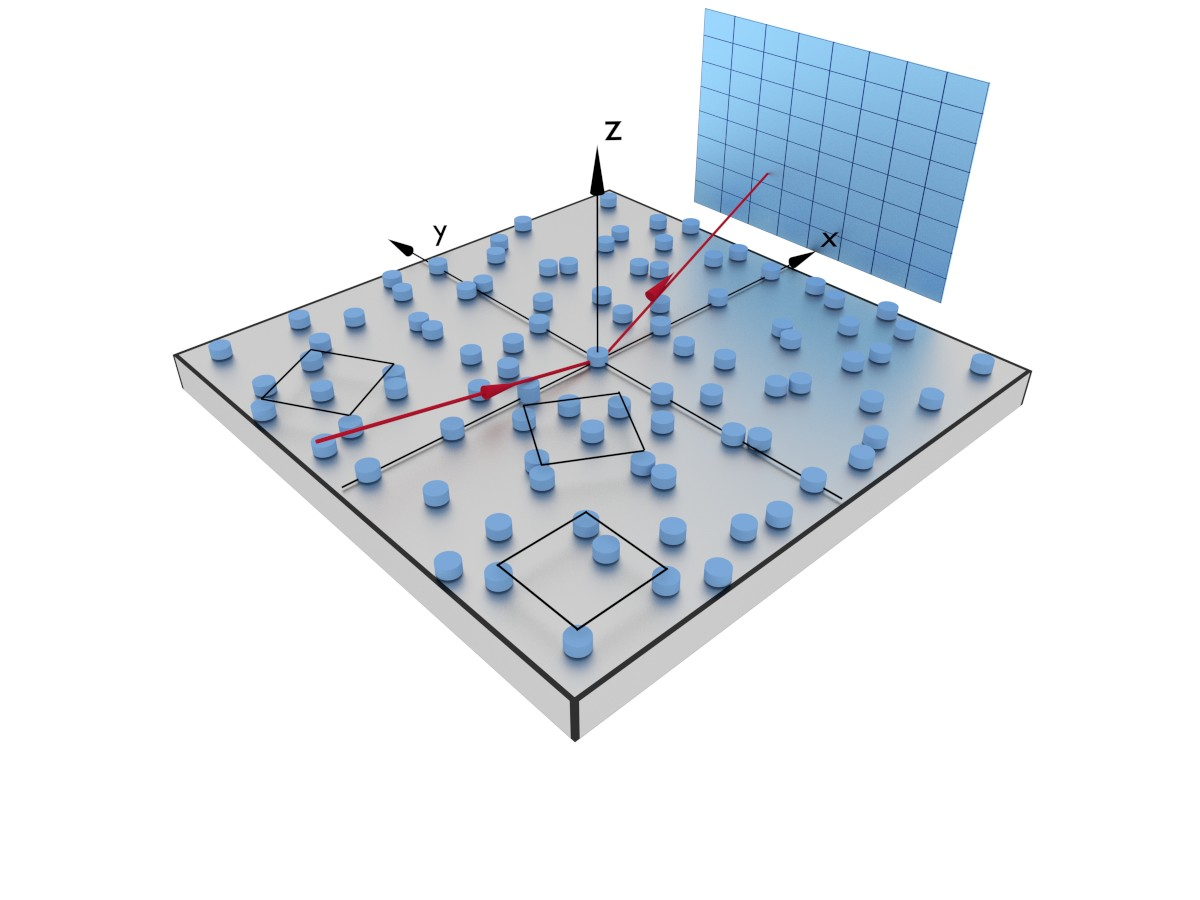
\includegraphics[width=.49\textwidth]{Figures/fig_ex005Dis4rand}}
\hfill
\subfigure[Simulated 2D pattern]{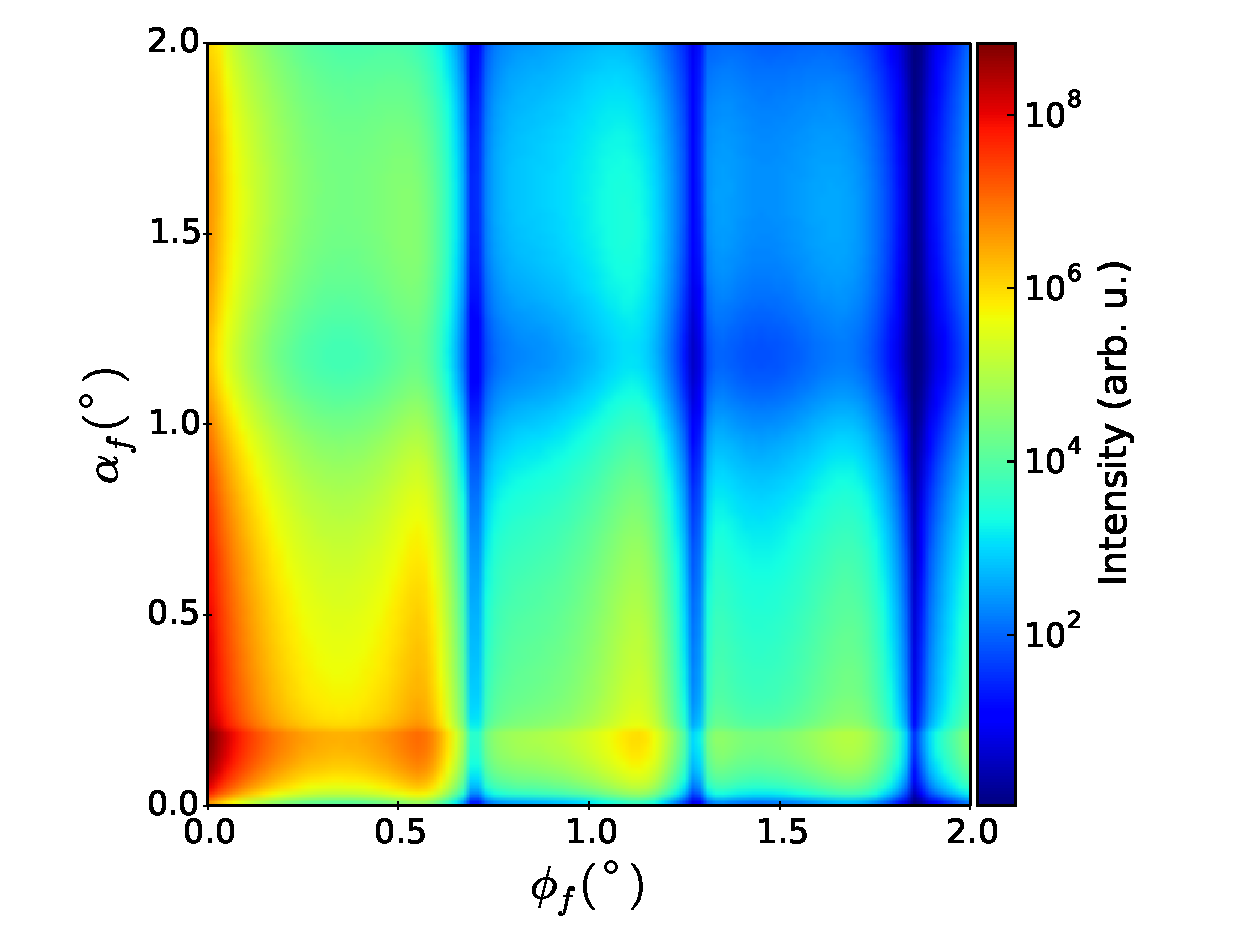
\includegraphics[width=.49\textwidth]{Figures/figure_ex005Disorder4.eps}}
\hfill
\caption{Example 005 - Disorder4: Scattering from a monodisperse distribution of cylinders deposited on a substrate.}
\label{fig:PythonEx5Dis4}
\end{figure}

\newpage
%%%%%%%%%%%%%%%%%%%%%%%%%%%%%%%
\section{Example 6: Rotated pyramids}
This example illustrates how the in-plane rotation of non-radially symmetric particles influences the scattering pattern. \\
The sample is made of pyramids (squared-base side length = 10~nm, height = 5~nm, $\alpha=54.73^{\circ}$, see \SecRef{Pyramid}) deposited on a substrate. There is no interference.\\
The wavelength is 1~\AA. The incident angles are $\alpha_i=0.2^{\circ}$ and $\phi_i=0^{\circ}$.\\
For the second example, shown in fig.~\ref{fig:PythonEx6RotatedPyramid}, the pyramids are rotated in the $(x,y)$ plane by 45$^{\circ}$.

\begin{figure}[H]
\hfill
\subfigure[Schematic of the sample]{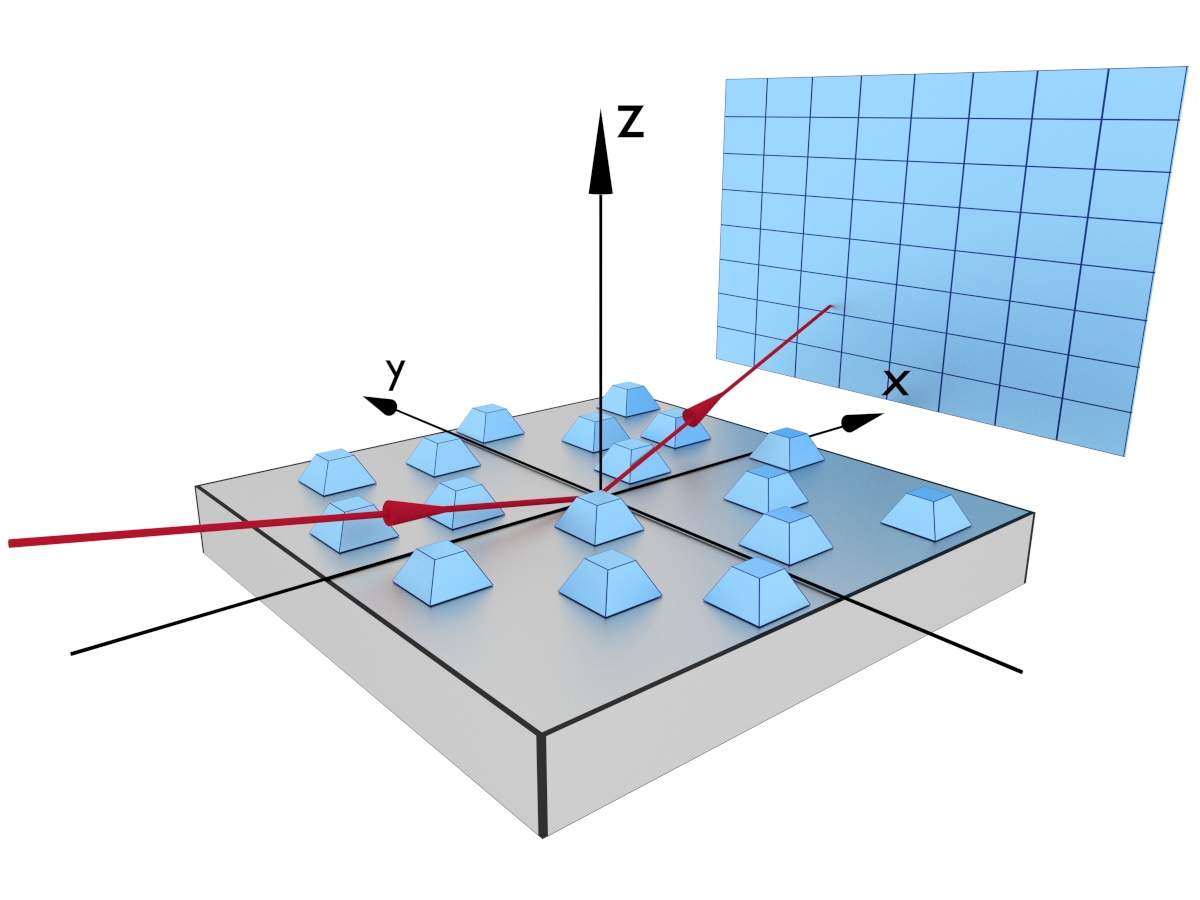
\includegraphics[width=.49\textwidth]{Figures/fig_ex006Pyramids}}
\hfill
\subfigure[Simulated 2D pattern]{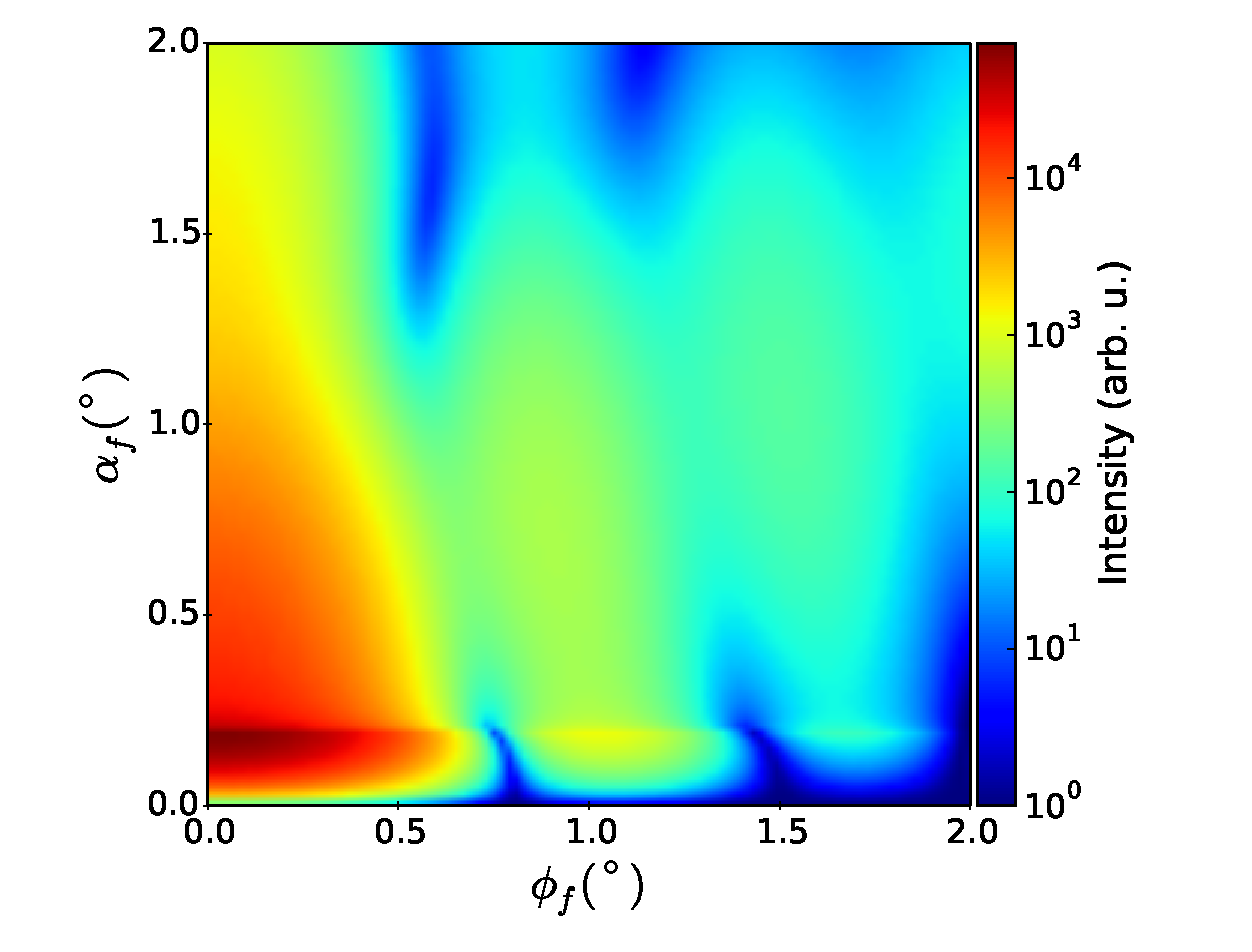
\includegraphics[width=.49\textwidth]{Figures/figure_ex006Pyramids.eps}}
\hfill
\caption{Example 6: Pyramids deposited on a substrate.}
\label{fig:PythonEx6Pyramid}
\end{figure}

\begin{figure}[H]
\hfill
\subfigure[Schematic of the sample]{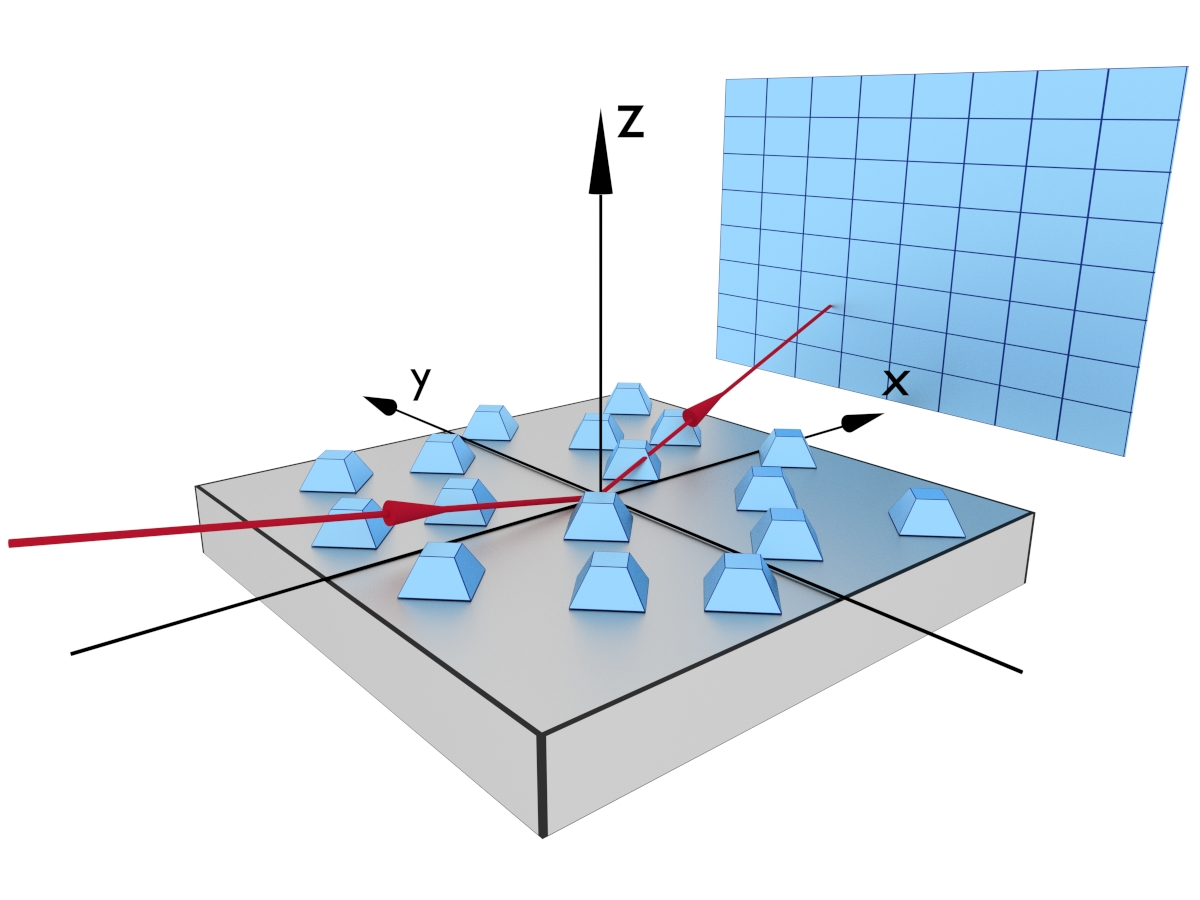
\includegraphics[width=.49\textwidth]{Figures/fig_ex006RotatedPyramids}}
\hfill
\subfigure[Simulated 2D pattern]{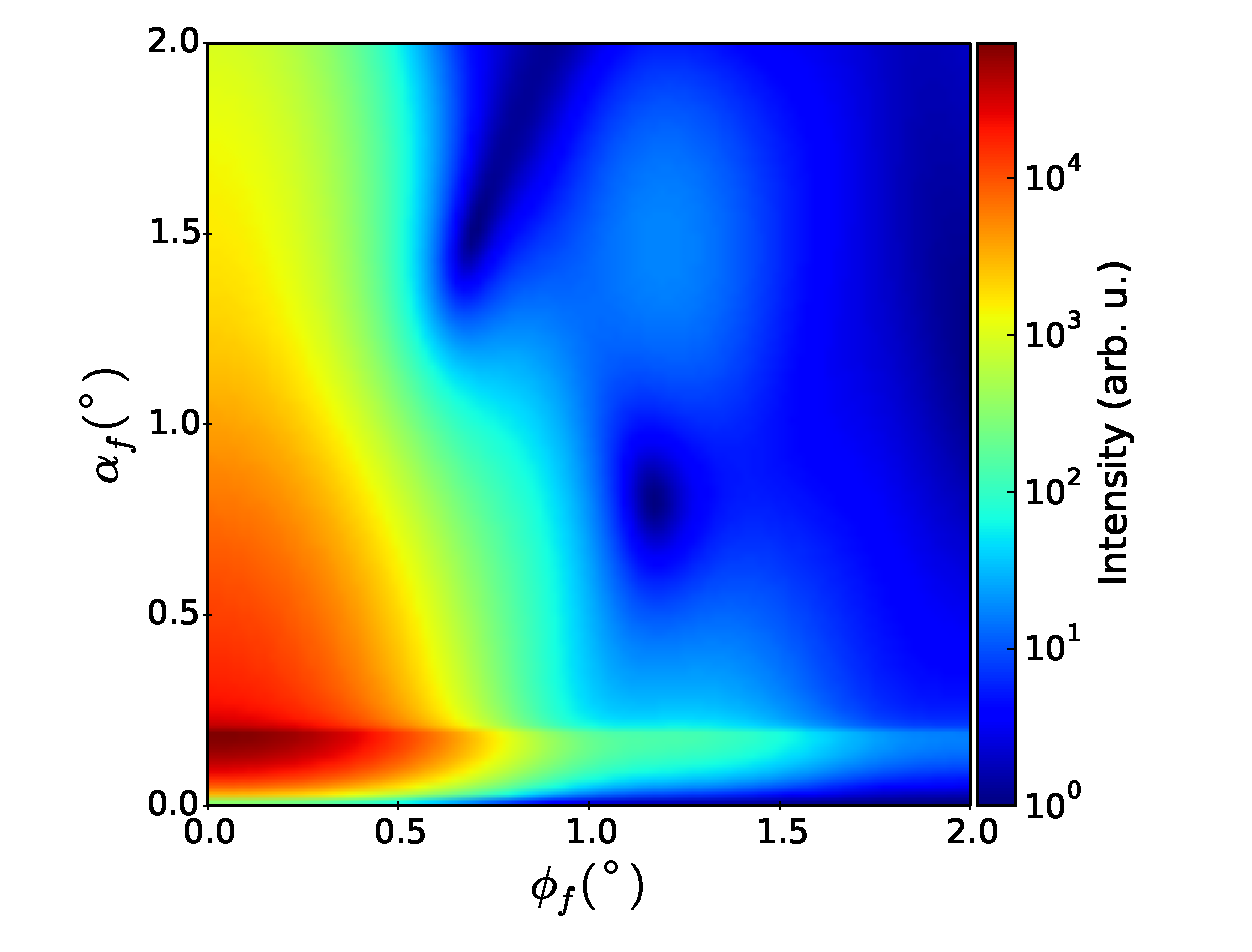
\includegraphics[width=.49\textwidth]{Figures/figure_ex006RotatedPyramids.eps}}
\hfill
\caption{Example 6: Rotated pyramids deposited on a substrate.}
\label{fig:PythonEx6RotatedPyramid}
\end{figure}

\newpage
%%%%%%%%%%%%%%%%%%%%%%%%%%%%%%%
\section{Example 7: Core-shell nanoparticles}
The sample is made of core-shell particles whose inner and outer shells are parallelepipeds with dimensions  $L_1=W_1=16$~nm, $H_1=8$~nm and  $L_2=W_2=12$~nm, $H_2=7$~nm, respectively, where $L_i$, $W_i$, and $H_i$ are the length, width and height of box $i$ (see fig.~\ref{fig:PythonEx7Core}). The smaller box is positioned so that the centres of the bottom faces of both particles coincide (see \ref{subsec:CoreShell} for details about this form factor). 

The simulation is run using the Born approximation. There is no substrate and no interference between the different scattered beams.

The incident beam is characterized by a wavelength of 1~\AA, incident angles $\alpha_i=0.2^{\circ}$ and $\phi_i=0^{\circ}$.


\begin{figure}[H]
\hfill
\subfigure[Schematic of the sample]{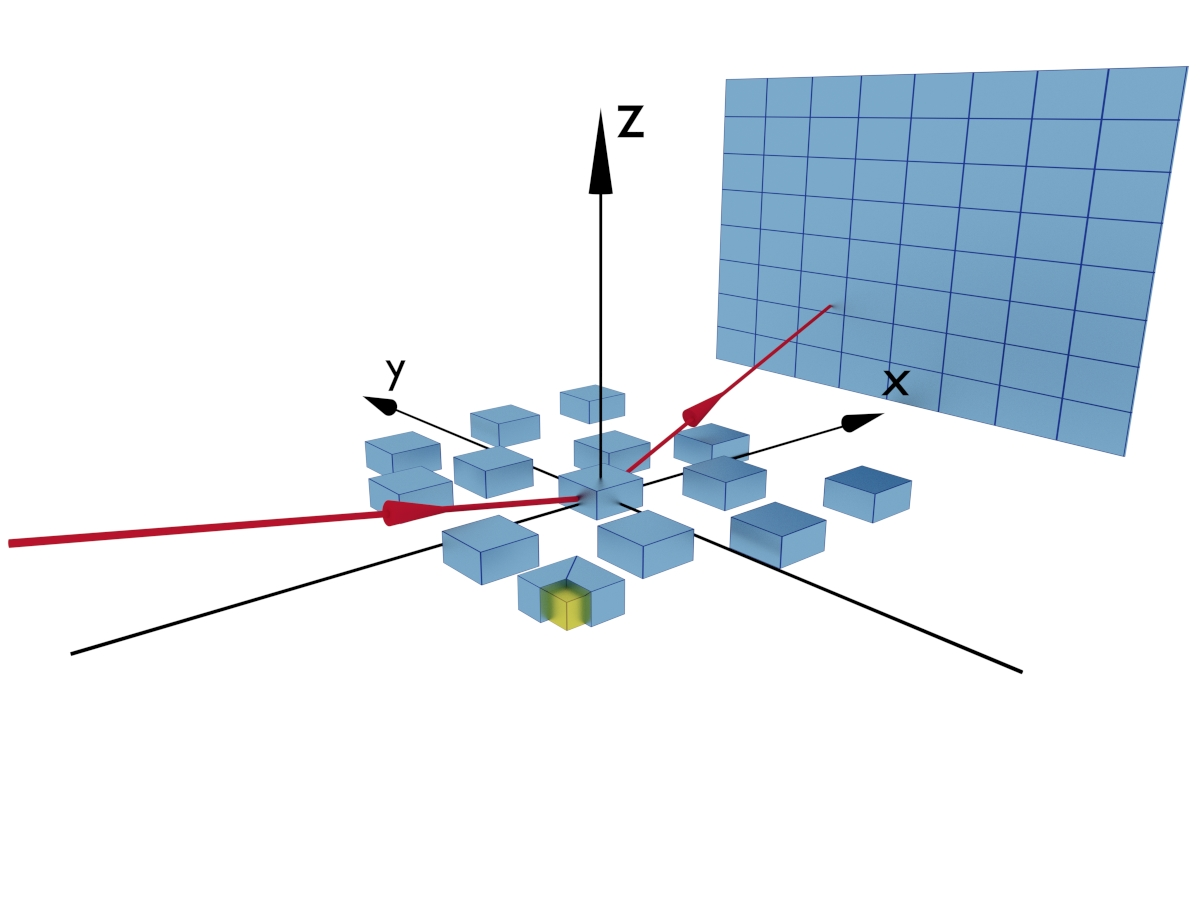
\includegraphics[width=.49\textwidth]{Figures/fig_ex007Core}}
\hfill
\subfigure[Simulated 2D pattern]{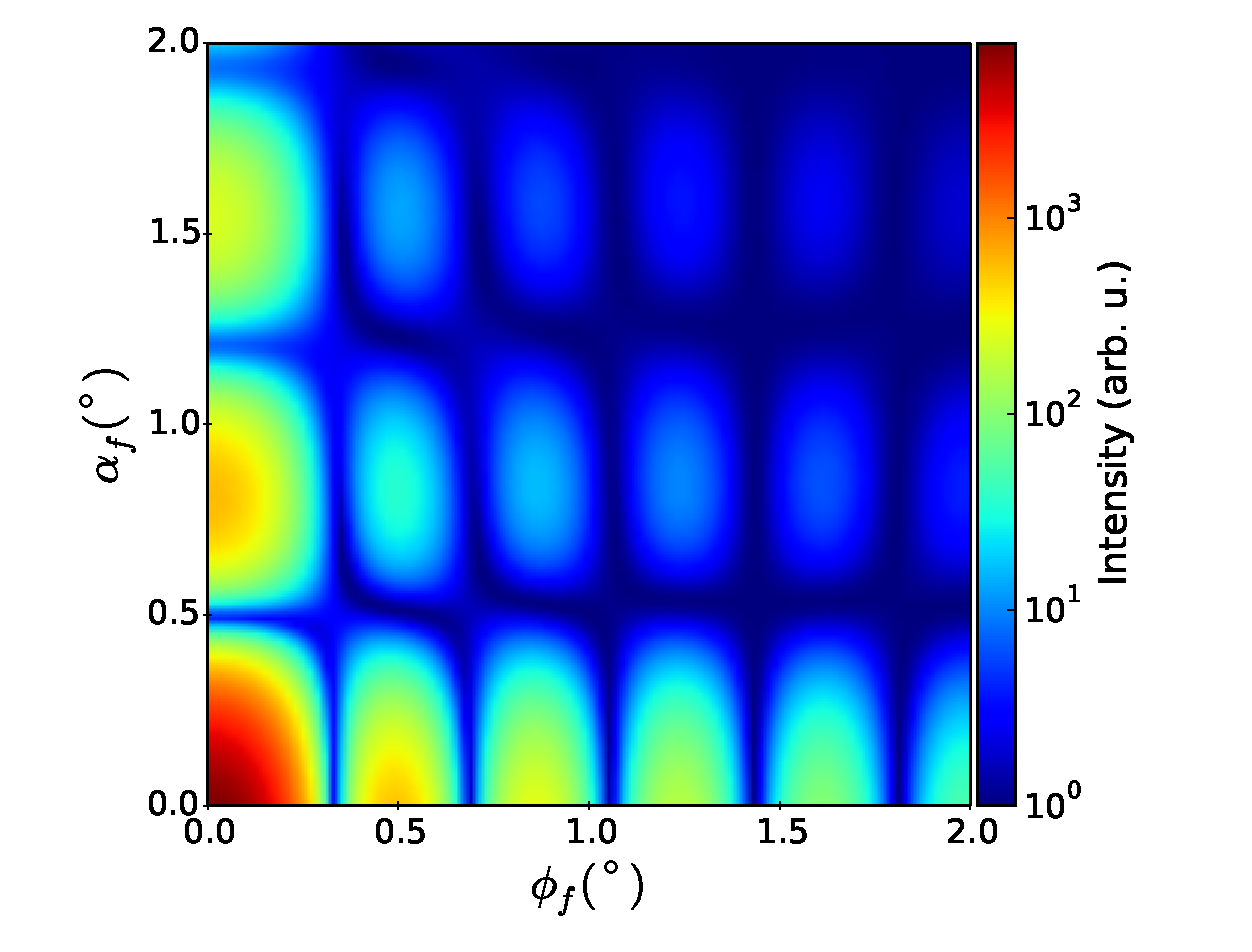
\includegraphics[width=.49\textwidth]{Figures/figure_ex007CoreShell.eps}}
\hfill
\caption{Example 7: Core-shell particles simulated using the Born approximation. The particle at the forefront had been truncated in order to illustrate the core-shell structure.}
\label{fig:PythonEx7Core}
\end{figure}

\newpage
%%%%%%%%%%%%%%%%%%%%%%%%%%%%%%%
\section{Example 8: Correlated roughness}
The sample is made in the following way from top to bottom: 

\begin{itemize}
    \item \ntikzmark{L}{layer A: A: 2.5~nm-thick, $n=1-5e-6$.}
    \item \ntikzmark{O}{layer B:  5~nm-thick, $n=1-1e-5$.}
    \item substrate: infinitely thick, $n=1-15e-6$
\end{itemize}
\makebrace{L}{O}{$\times$ 5.}

There is no added particle. All layers present the same type of roughness on the top surface, which is characterized by
\begin{itemize}
\item $\sigma=1$~nm,
\item a Hurst parameter $H$ equal to 0.3,
\item a lateral correlation length $\xi$ of 5~nm,
\item a cross correlation length $\xi_{\perp}$ equal to 1e-4~nm.
\end{itemize}

\MakeRemark{Roughness in \BornAgain}{The implementation is based on Reference~\cite{Boer95,Schlomka95}.\\ The roughness profile is described by a normally-distributed random function. The roughness correlation function at j$^\textrm{th}$ interface is expressed as  $\langle U_j(x,y) U_j(x',y') \rangle = \sigma^2 \exp(-(\tau/\xi)^{2H})$,
 $\tau=\sqrt{(x-x')^2+(y-y')^2}$, where $U_j(x,y)$ is the height deviation of the j$^{\textrm{th}}$ interface at position $(x,y)$.
\\ $\sigma$ gives the rms roughness of the interface.\\ The Hurst parameter $H$, comprised between 0 and 1 is connected to the fractal dimension $D=3-H$ of the interface. The smaller $H$ is, the more serrate the surface profile looks. If $H=1$, the interface has a non fractal nature.\\ The lateral correlation length $\xi$ acts as a cut-off for the lateral length scale on which an interface begins to look smooth. If $\xi >> \tau$ the surface looks smooth.\\ The cross correlation length $\xi_{\perp}$ is the vertical distance over which the correlation between layers is damped by a factor $1/e$. It is assumed to be the same for all interfaces. If $\xi_{\perp}=0$ there is no correlations between layers. If $\xi_{\perp}$ is much larger than the layer thickness, the layers are perfectly correlated.}

The incident beam is characterized by a wavelength of 1~\AA \ and incident angles $\alpha_i=0.2^{\circ}$ and $\phi_i=0^{\circ}$. 
\begin{figure}[H]
\hfill
\subfigure[Schematic of the sample]{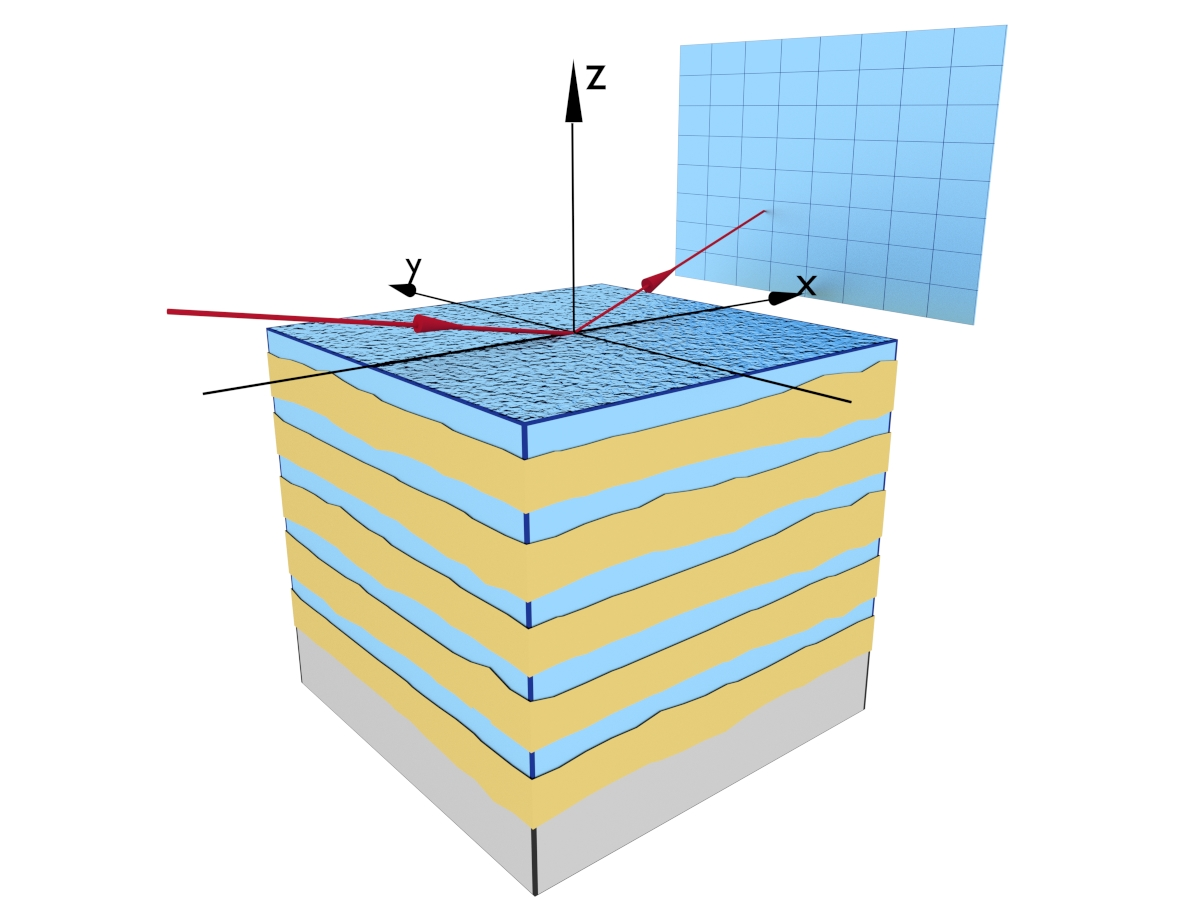
\includegraphics[width=.49\textwidth]{Figures/fig_ex008Rough}}
\hfill
\subfigure[Simulated 2D pattern]{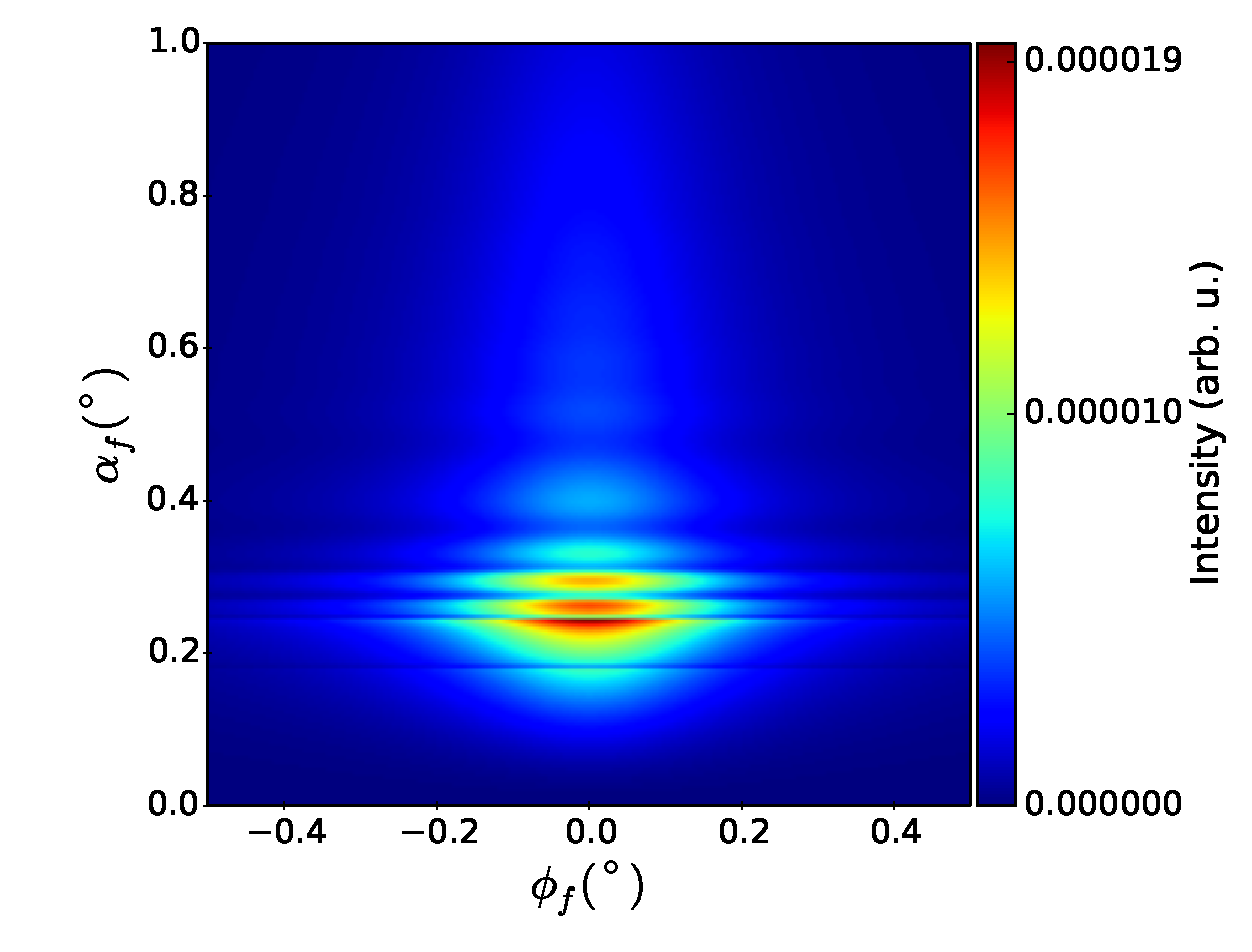
\includegraphics[width=.49\textwidth]{Figures/figure_ex008CorrelatedRough.eps}}
\hfill
\caption{Example 8: Correlated roughness between layers.}
\label{fig:PythonEx8Rough}
\end{figure}

%Power spectral density of the surface roughness is a result of two-dimensional
%Fourier transform of the correlation function of the roughness profile.
% Based on the article D.K.G. de Boer, Physical review B, Volume 51, Number 8, 15 February 1995 "X-ray reflection and transmission by rough surfaces"
 
\newpage
%%%%%%%%%%%%%%%%%%%%%%%%%%%%%%%
\section{Example 9: Ripple}
These particles have one of their dimensions much larger than the others.
Two different transverse profiles are simulated: one cosine and one asymmetric triangular.
These particles are deposited on a substrate. The input beam is characterized by a wavelength of 1.6~\AA and angles $\alpha_i=0.3^{\circ}$, $\phi_i=0^{\circ}$.

\subsection{Cosine ripple}
The particles have a cosine cross section (see \SecRef{Ripple1} for an illustration) with $L=100$~nm, $W=20$~nm, $H=4$~nm.
The interference considered is a two-dimensional orthogonal lattice with $L_1=200$~nm, $L_2=50$~nm. The rod shape distribution is an anisotropic 2D Gaussian with $cl_x=1000/(2\pi)$~nm and  $cl_y=100/(2\pi)$~nm.

\begin{figure}[H]
\hfill
\subfigure[Schematic of the sample]{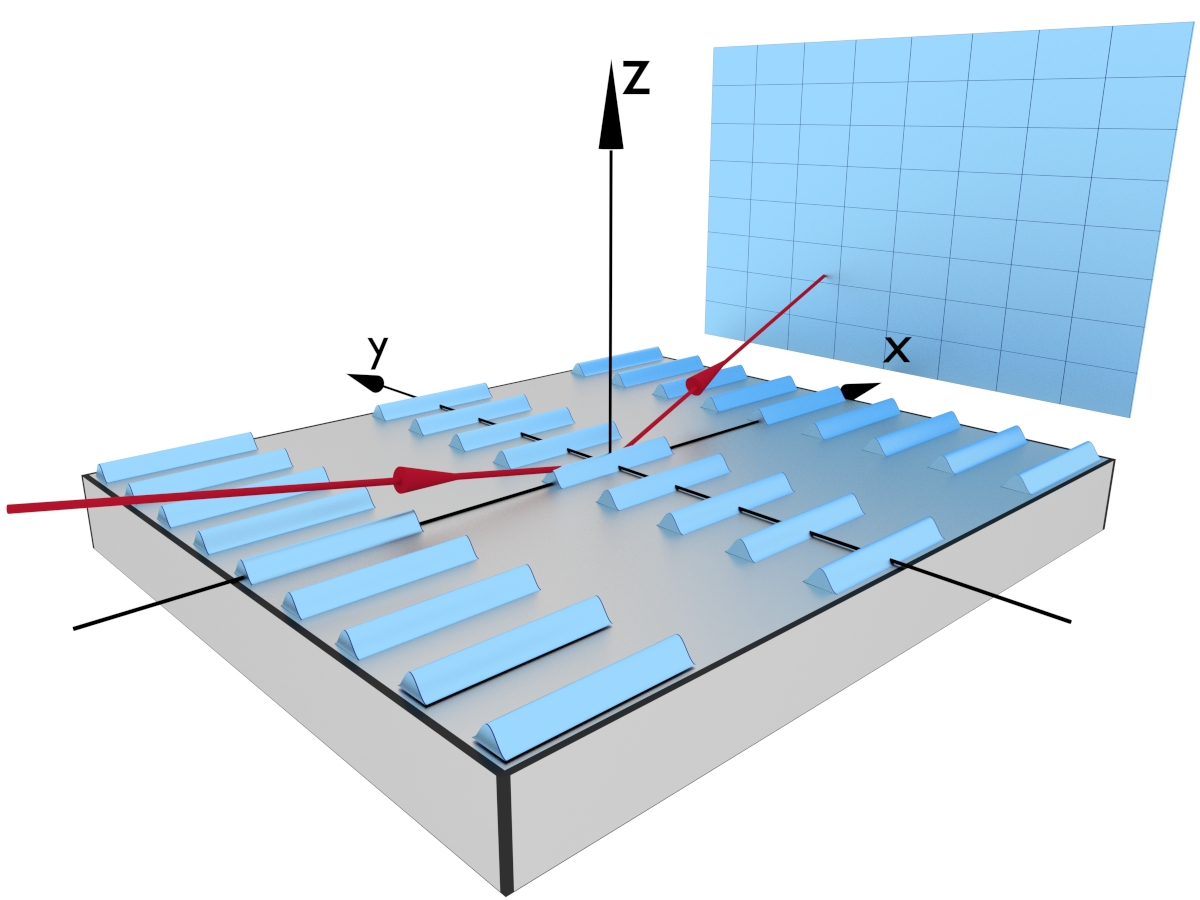
\includegraphics[width=.49\textwidth]{Figures/fig_ex009Cos}}
\hfill
\subfigure[Simulated 2D pattern]{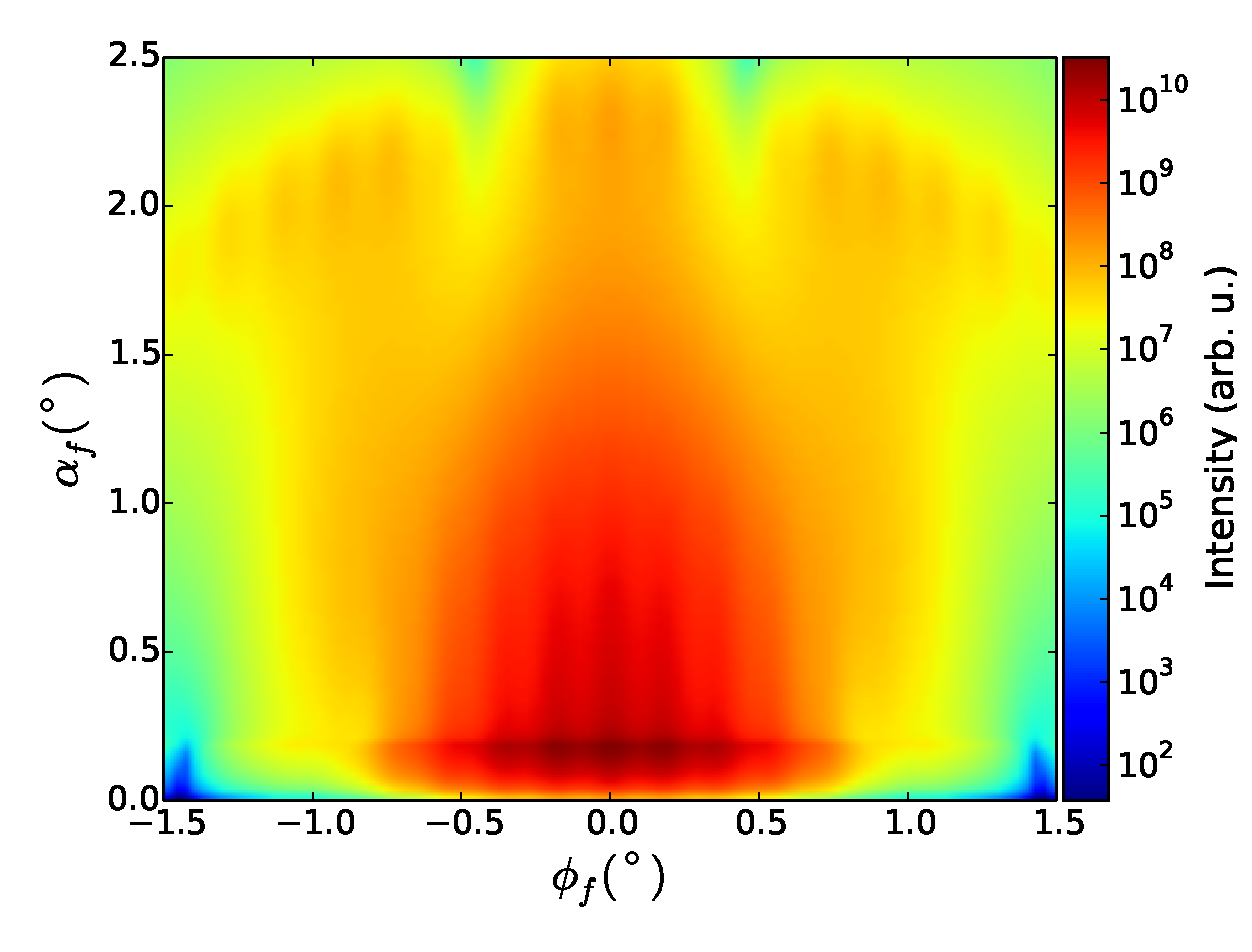
\includegraphics[width=.49\textwidth]{Figures/figure_ex009CosRipple2DLat.eps}}
\hfill
\caption{Example 9: Scattering from a distribution of cosine ripples deposited on a substrate along a rectangular lattice.}
\label{fig:PythonEx9CosRipple}
\end{figure}

The influence of the interference function on the output pattern can be seen by comparing figures~\ref{fig:PythonEx9CosRipple}(b) and \ref{fig:PythonEx9CosRipplenointerf}. The latter has been generated without any interference (\textit{i.e.} with a diluted distribution of particles).

\begin{figure}[H]
\begin{center}
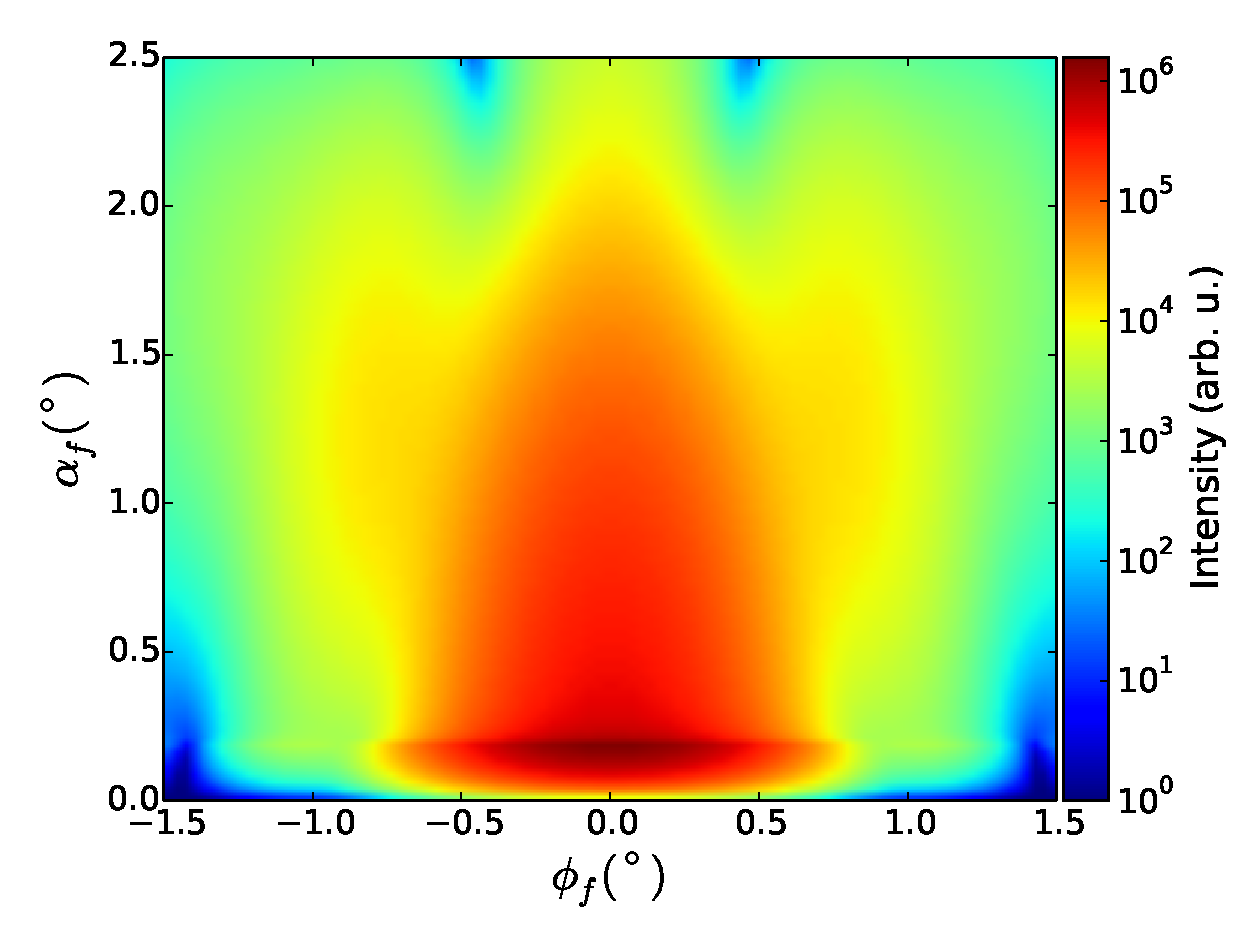
\includegraphics[width=0.5\textwidth]{Figures/figure_ex009CosRippleNoInterf.eps}
\end{center}
\caption{Example 9: Scattering from a distribution of cosine ripples deposited on a substrate with no interference.}
\label{fig:PythonEx9CosRipplenointerf}
\end{figure}

\subsection{Triangular ripple}
 The particles are long particles with an asymmetric triangular cross section (see \SecRef{Ripple2}) with  $L=100$~nm, $W=20$~nm, $H=4$~nm, an asymmetry coefficent of $-3$~nm. The interference function has the same characteristics as in the previous example.

\begin{figure}[H]
\hfill
\subfigure[Schematic of the sample]{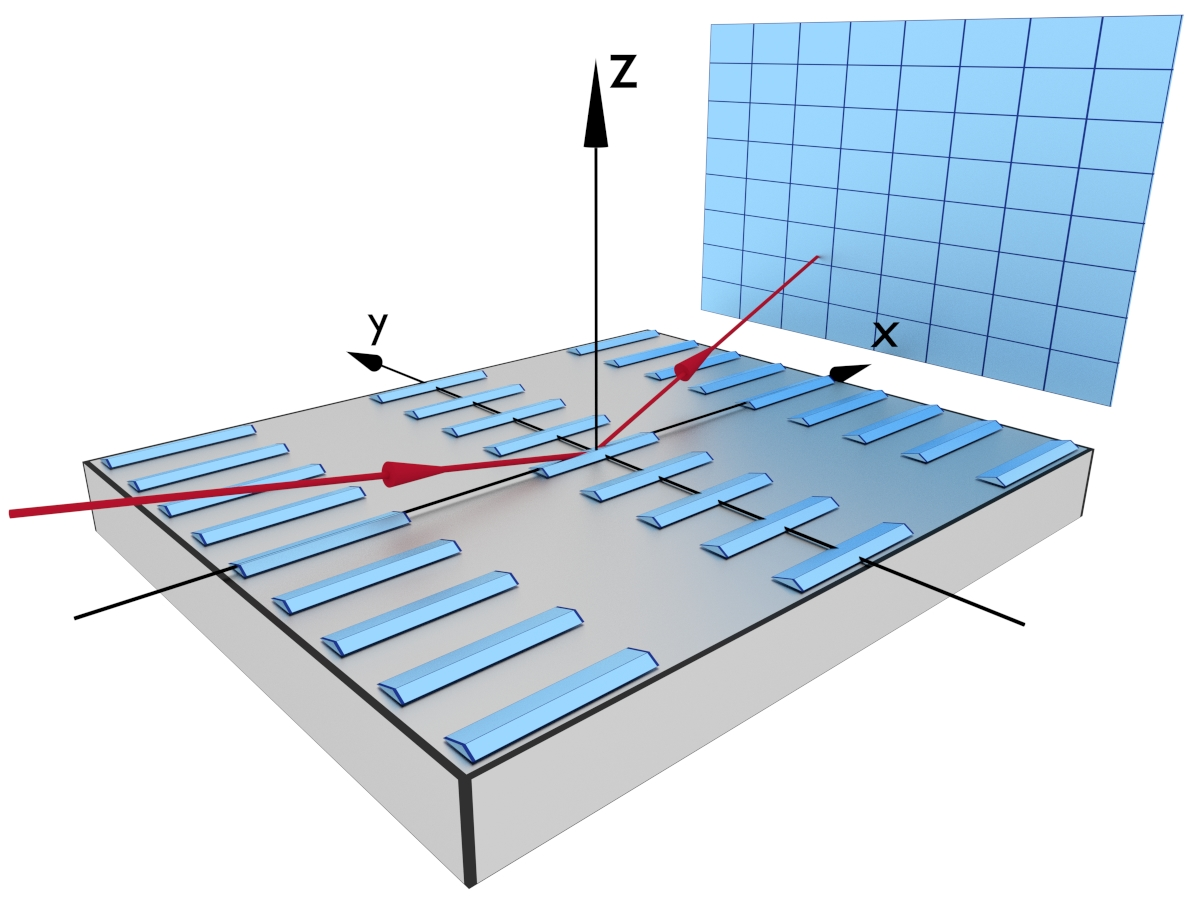
\includegraphics[width=.49\textwidth]{Figures/fig_ex009Tri}}
\hfill
\subfigure[Simulated 2D pattern]{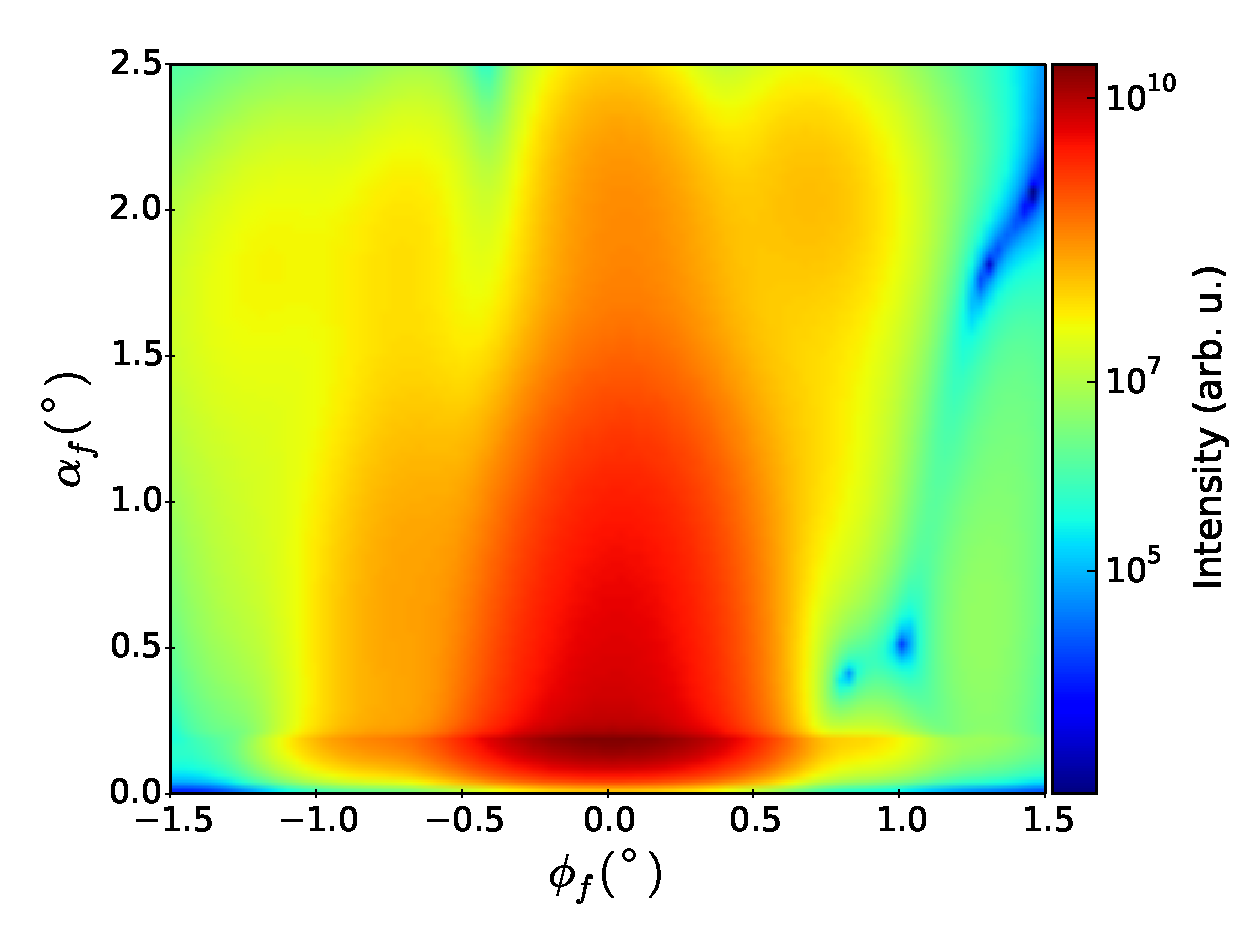
\includegraphics[width=.49\textwidth]{Figures/figure_ex009TriRipple2DLat.eps}}
\hfill
\caption{Example 9: Scattering from a distribution of triangular ripples deposited on a substrate with no interference.}
\label{fig:PythonEx9TriangRipple}
\end{figure}

Figure~\ref{fig:PythonEx9TriRipplenointerf} was generated with asymmetrical triangular ripples but with no interference. It therefore illustrates the influence of the particle's shape on the scattering pattern.

\begin{figure}[H]
\begin{center}
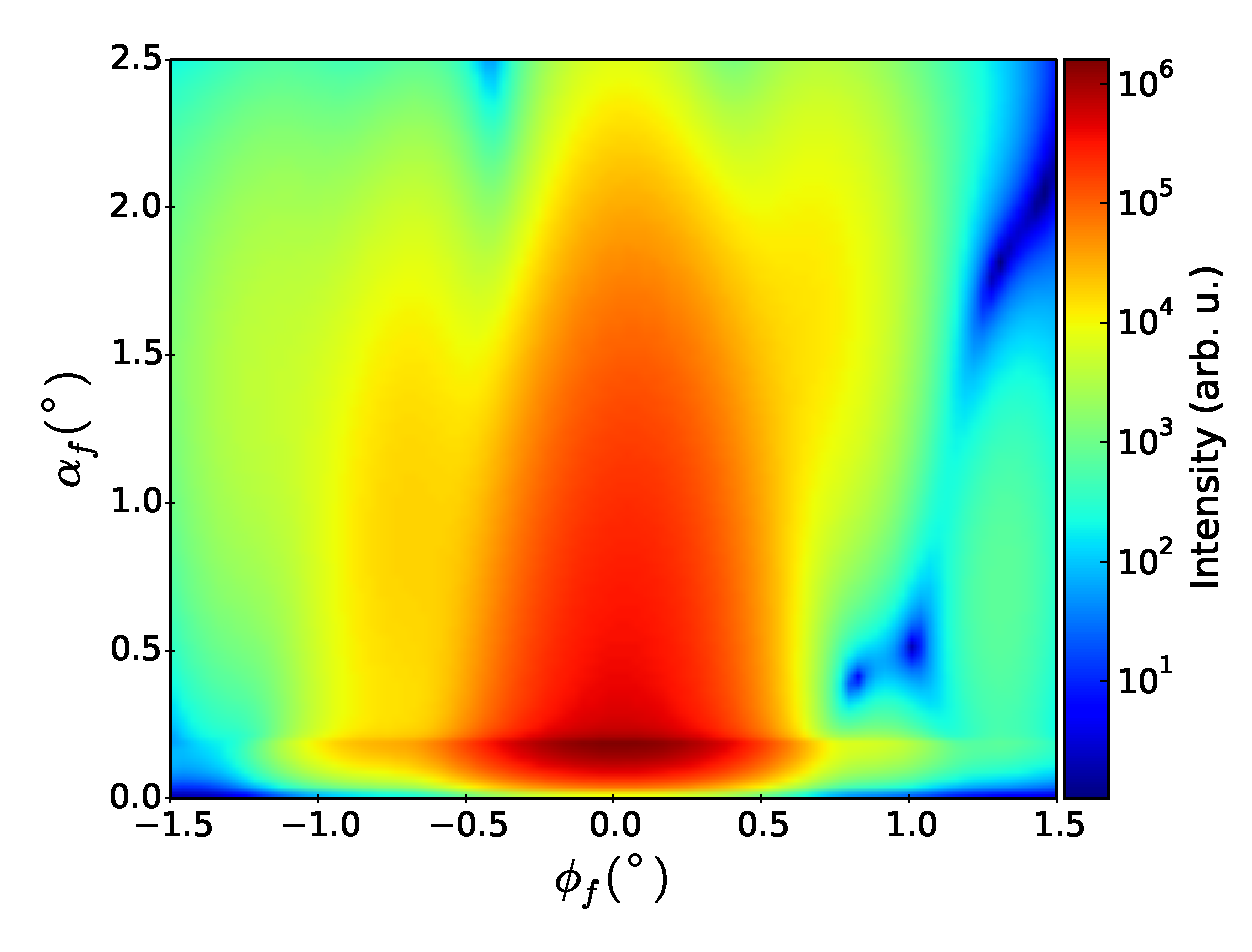
\includegraphics[width=0.5\textwidth]{Figures/figure_ex009TriRippleNoInterf.eps}
\end{center}
\caption{Example 9: Scattering from a distribution of triangular ripples deposited on a substrate with no interference.}
\label{fig:PythonEx9TriRipplenointerf}
\end{figure}

\newpage
%%%%%%%%%%%%%%%%%%%%%%%%%%%%%%%
\section{Example 10: Beam divergence}
The main point of this example is the input beam, which presents a divergence for:
\begin{itemize}
\item the wavelength, following a log-normal distribution around the mean value of 1~\AA\ with a scale parameter equal to 0.1 (see the remark at the end of this section for a definition of these parameters).
\item  both incident angles following a Gaussian distribution with 
$\bar \alpha_i=0.2^{\circ}$, $\bar\phi_i=0^{\circ}$ and $\sigma_{\alpha_i}=\sigma_{\phi_i}=0.1^{\circ}$.
\end{itemize}
The sample is made of cylinders (5~nm in radius and height) deposited on a substrate, whose scattered beams do not interfere (fig.~\ref{fig:PythonEx10BeamDiv}(a)). The simulation is run using the Distorted Wave Born Approximation.

\begin{figure}[H]
\hfill
\subfigure[Schematic of the sample]{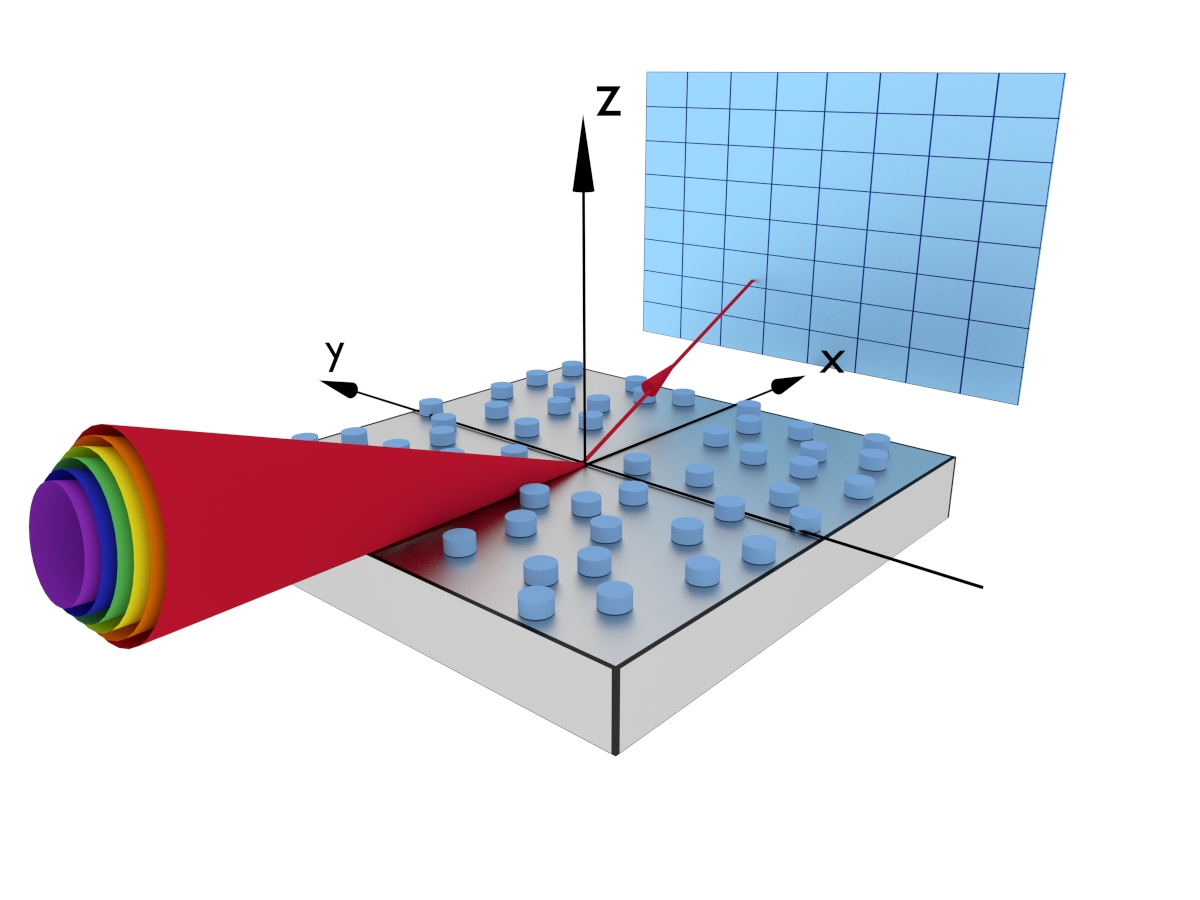
\includegraphics[width=.49\textwidth]{Figures/fig_ex010BeamDiv}}
\hfill
\subfigure[Simulated 2D pattern]{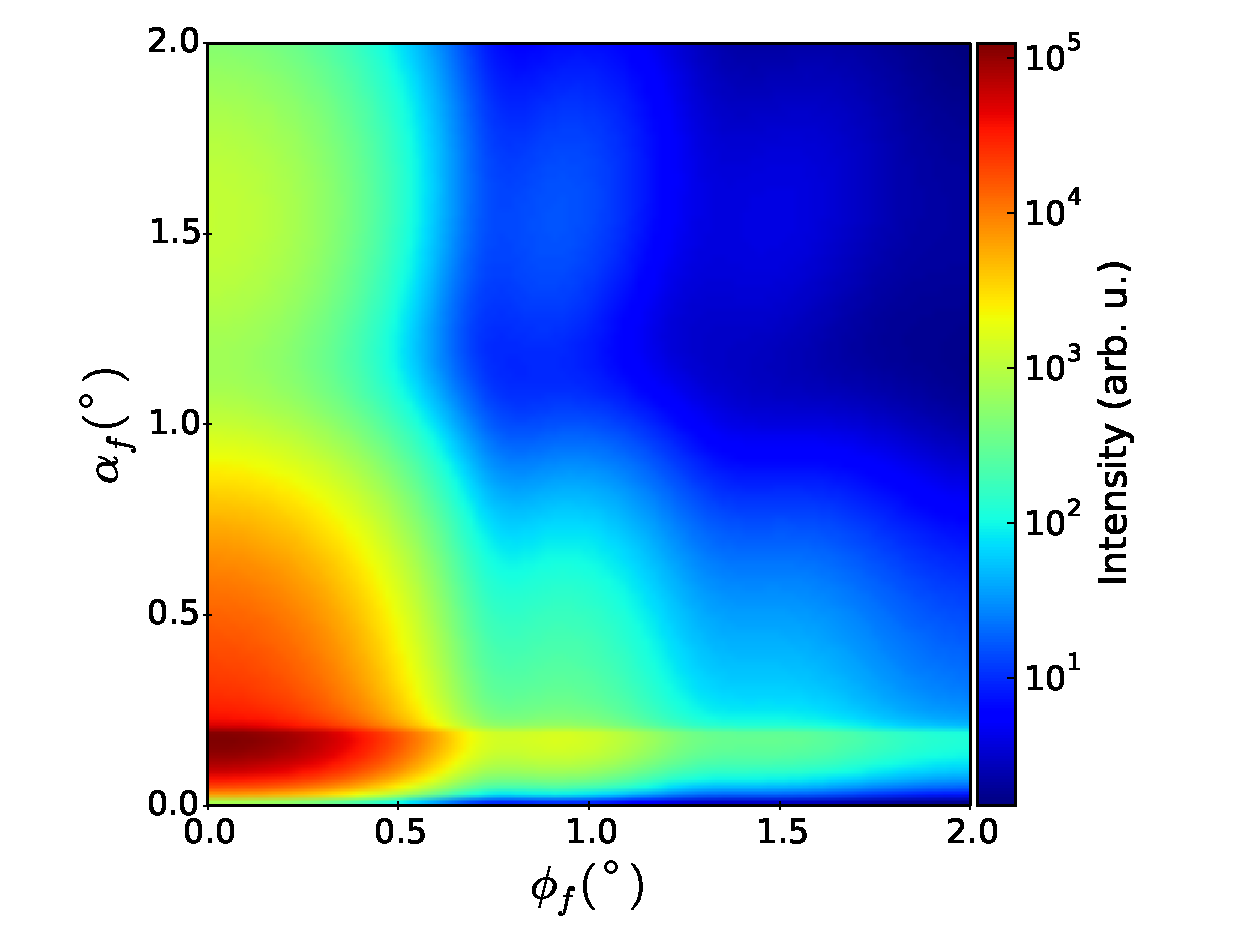
\includegraphics[width=.49\textwidth]{Figures/figure_ex010BeamDiv.eps}}
\hfill
\caption{Example 10: An input beam presented a divergence for the wavelength and the incident angles impinges on a sample made of monodisperse cylinders deposited on a substrate.}
\label{fig:PythonEx10BeamDiv}
\end{figure}

This example and the one presented in Section~\ref{sec:ex003CylinderDWBA} differ only by the divergence of the input beam. Comparing the output patterns shows that the largest impact of input beam divergence is a reduction of the sharpness in the intensity pattern for larger values of $\phi_f$ and $\alpha_f$.\\



\MakeRemark{Remark:}{The Gaussian distribution is characterised by 
$$p(\bar{x},\sigma)=\frac{1}{2\sigma^2}\exp\left[-\frac{(x-\bar{x})^2}{2\sigma^2} \right], $$
and the log-normal by
$$p(\textrm{median}, \textrm{scale})=\frac{1}{x\ \textrm{scale}\sqrt{2\pi}}\exp\left[-\frac{1}{2}\left( \frac{\log(x/\textrm{median})}{\textrm{scale}} \right)^2 \right].$$
}

